\documentclass[12pt]{article}
\usepackage[letterpaper, margin=1in]{geometry}
\usepackage{graphicx}
\graphicspath{{./Figures/}}
\usepackage{hyperref}
\usepackage{parskip}
\usepackage{amsmath}
\usepackage{caption}
\usepackage{subcaption}
\usepackage[framed, numbered]{matlab-prettifier}
\lstset{inputpath=../MATLAB}

\DeclareMathOperator{\sinc}{sinc}

\title{ELECENG 3TR4 Lab 3: \\ DSB-SC and QAM - Modulation and Demodulation}
\author{
    Aaron Pinto \\ pintoa9
    \and
    Raeed Hassan \\ hassam41
}

\begin{document}

\maketitle
\clearpage

\section*{Numerical Experiment 3.1: DSB-SC Signal}
The message signal is given by Equation~\ref{eq:dsbsc_message}, where $A_m$ = 1 V, $f_m$ = 1 kHz.
\begin{equation} \label{eq:dsbsc_message} 
    m(t) = A_m \cos(2 \pi f_m t)
\end{equation}
The DSB-SC signal is given by Equation~\ref{eq:dsbsc}, where $A_c$ = 1 V, and $f_c$ = 10 kHz.
\begin{equation} \label{eq:dsbsc}
    s(t) = A_c m(t) \cos(2 \pi f_c t)    
\end{equation}
The DSB-SC signal is plotted in the time domain in Figure~\ref{fig:dsbsc_time} and plotted in the frequency domain (magnitude spectrum) in Figure~\ref{fig:dsbsc_freq}. The MATLAB code used to generate the DSB-SC signal and its plots are found in the exp3\_1.m MATLAB script. A portion of the MATLAB code used to generate the DSB-SC signal, and the MATLAB code used to find the phase reversals are shown in Listing~\ref{listing:dsbsc}.
\lstinputlisting[style=Matlab-editor, caption={Generating the DSB-SC Signal}, label={listing:dsbsc}, linerange={18-27,146-162}]{exp3_1.m} 

\begin{figure}[h]
    \centering
    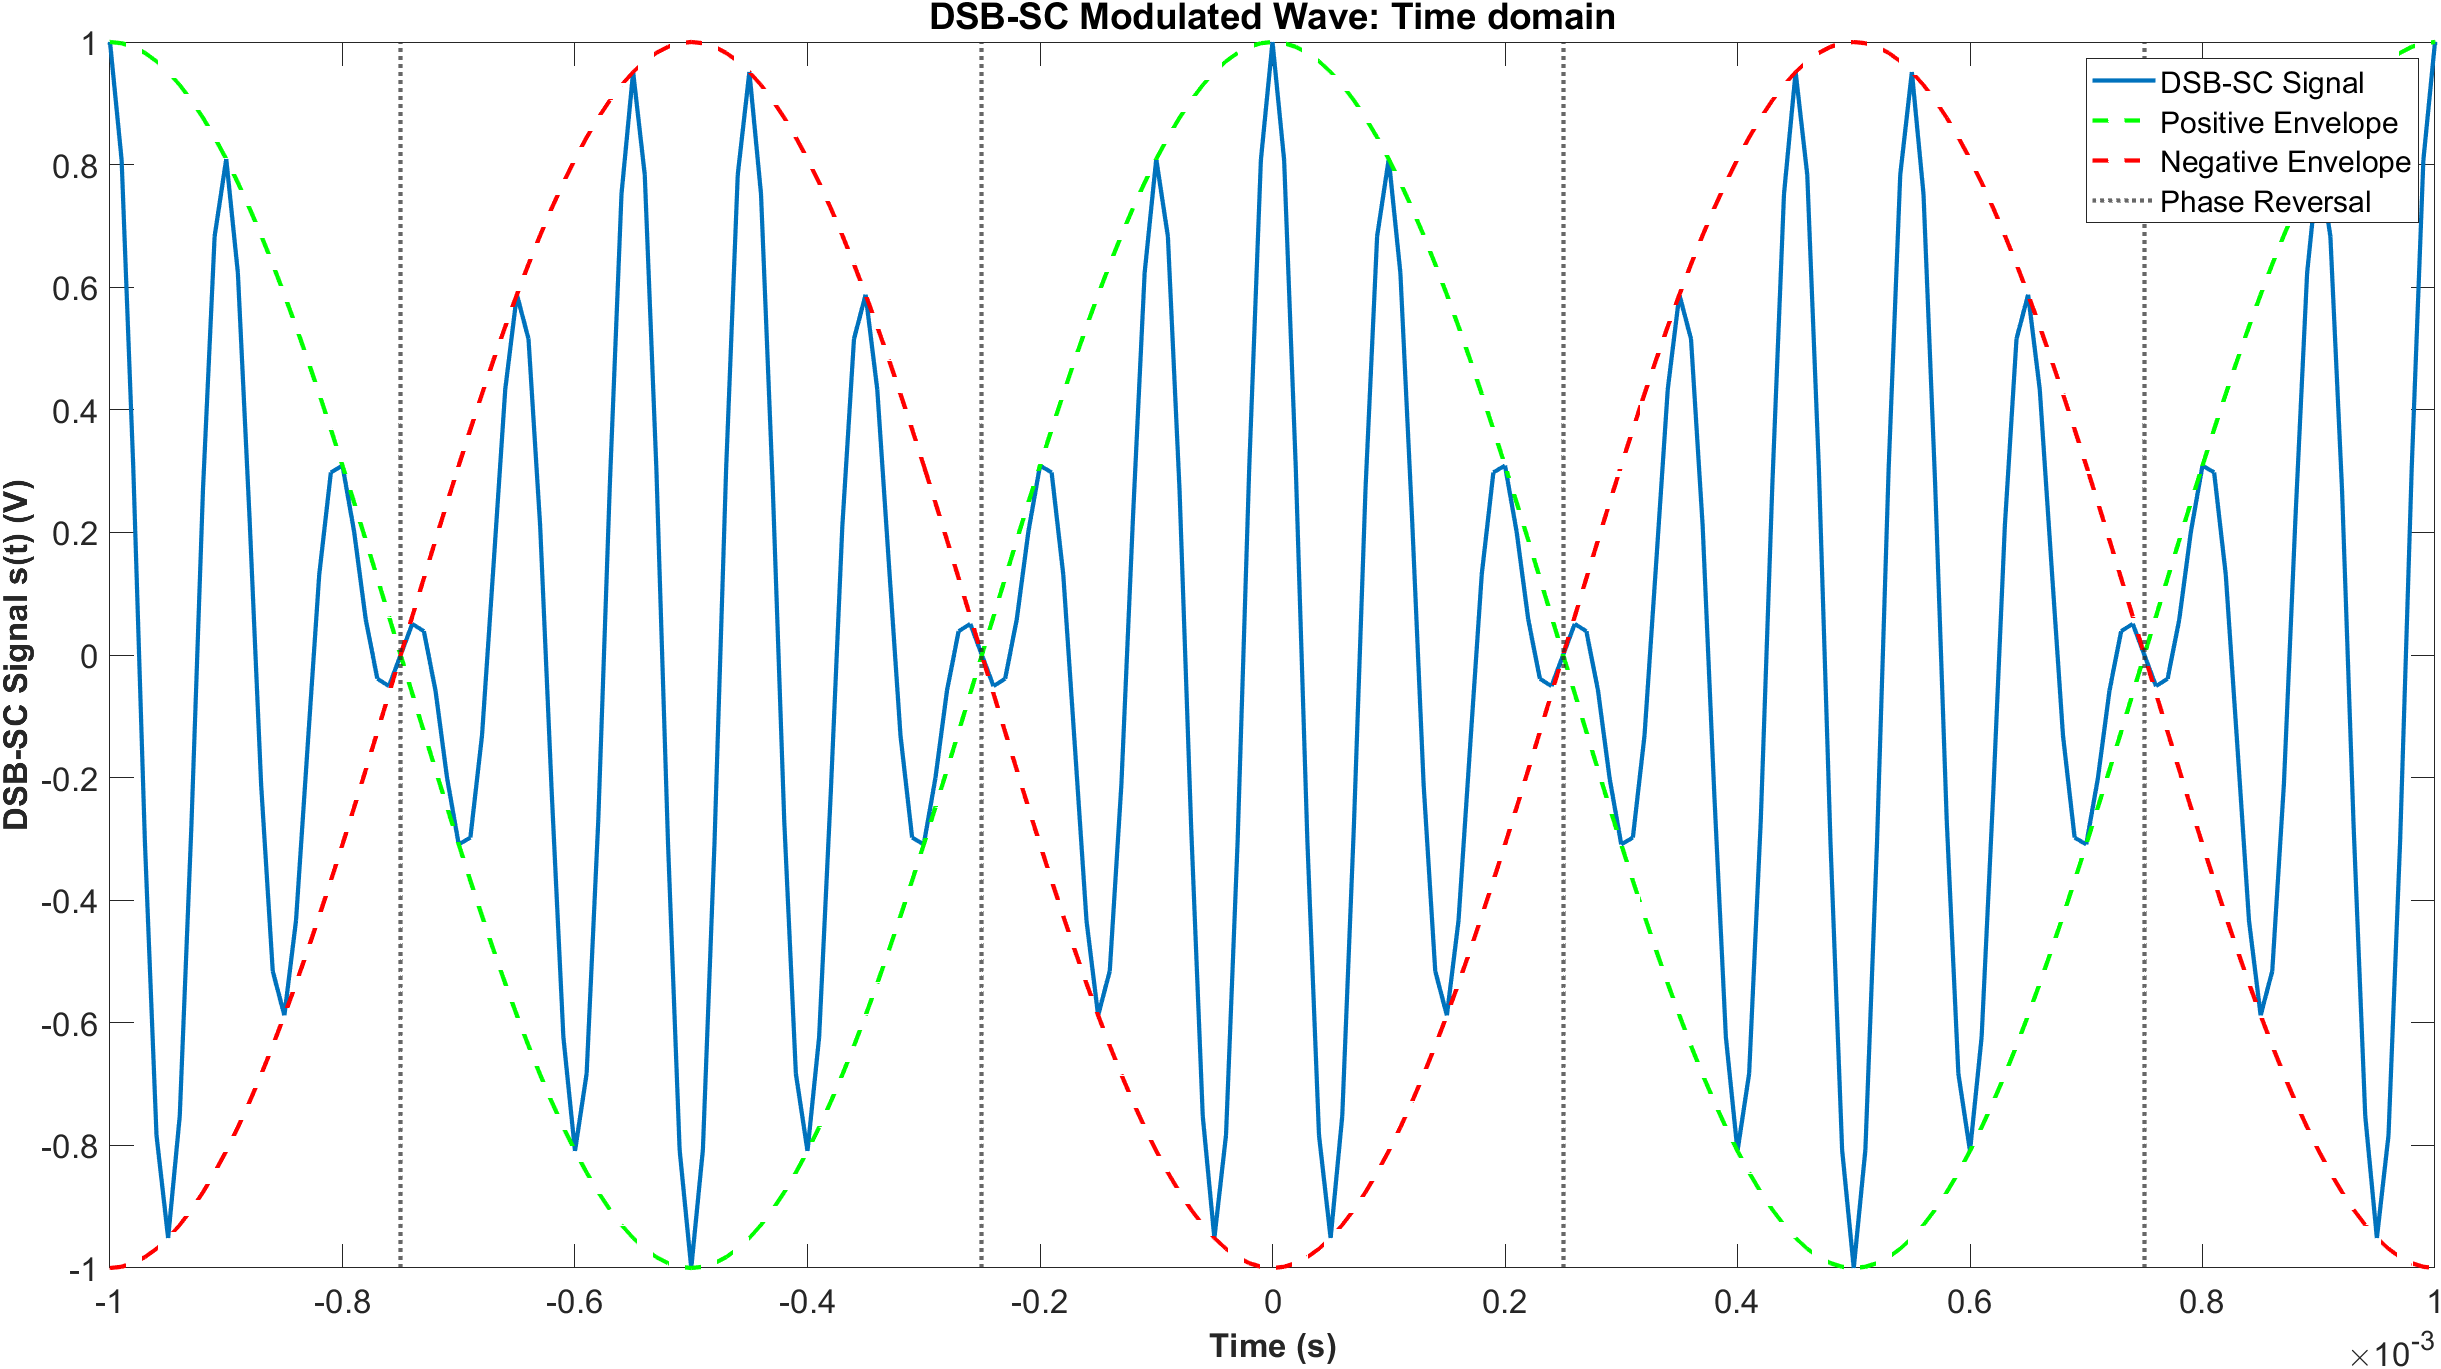
\includegraphics[width=\textwidth]{dsbsc_time}
    \caption{\label{fig:dsbsc_time}The DSB-SC Signal in Time Domain}
\end{figure}
\begin{figure}[h]
    \centering
    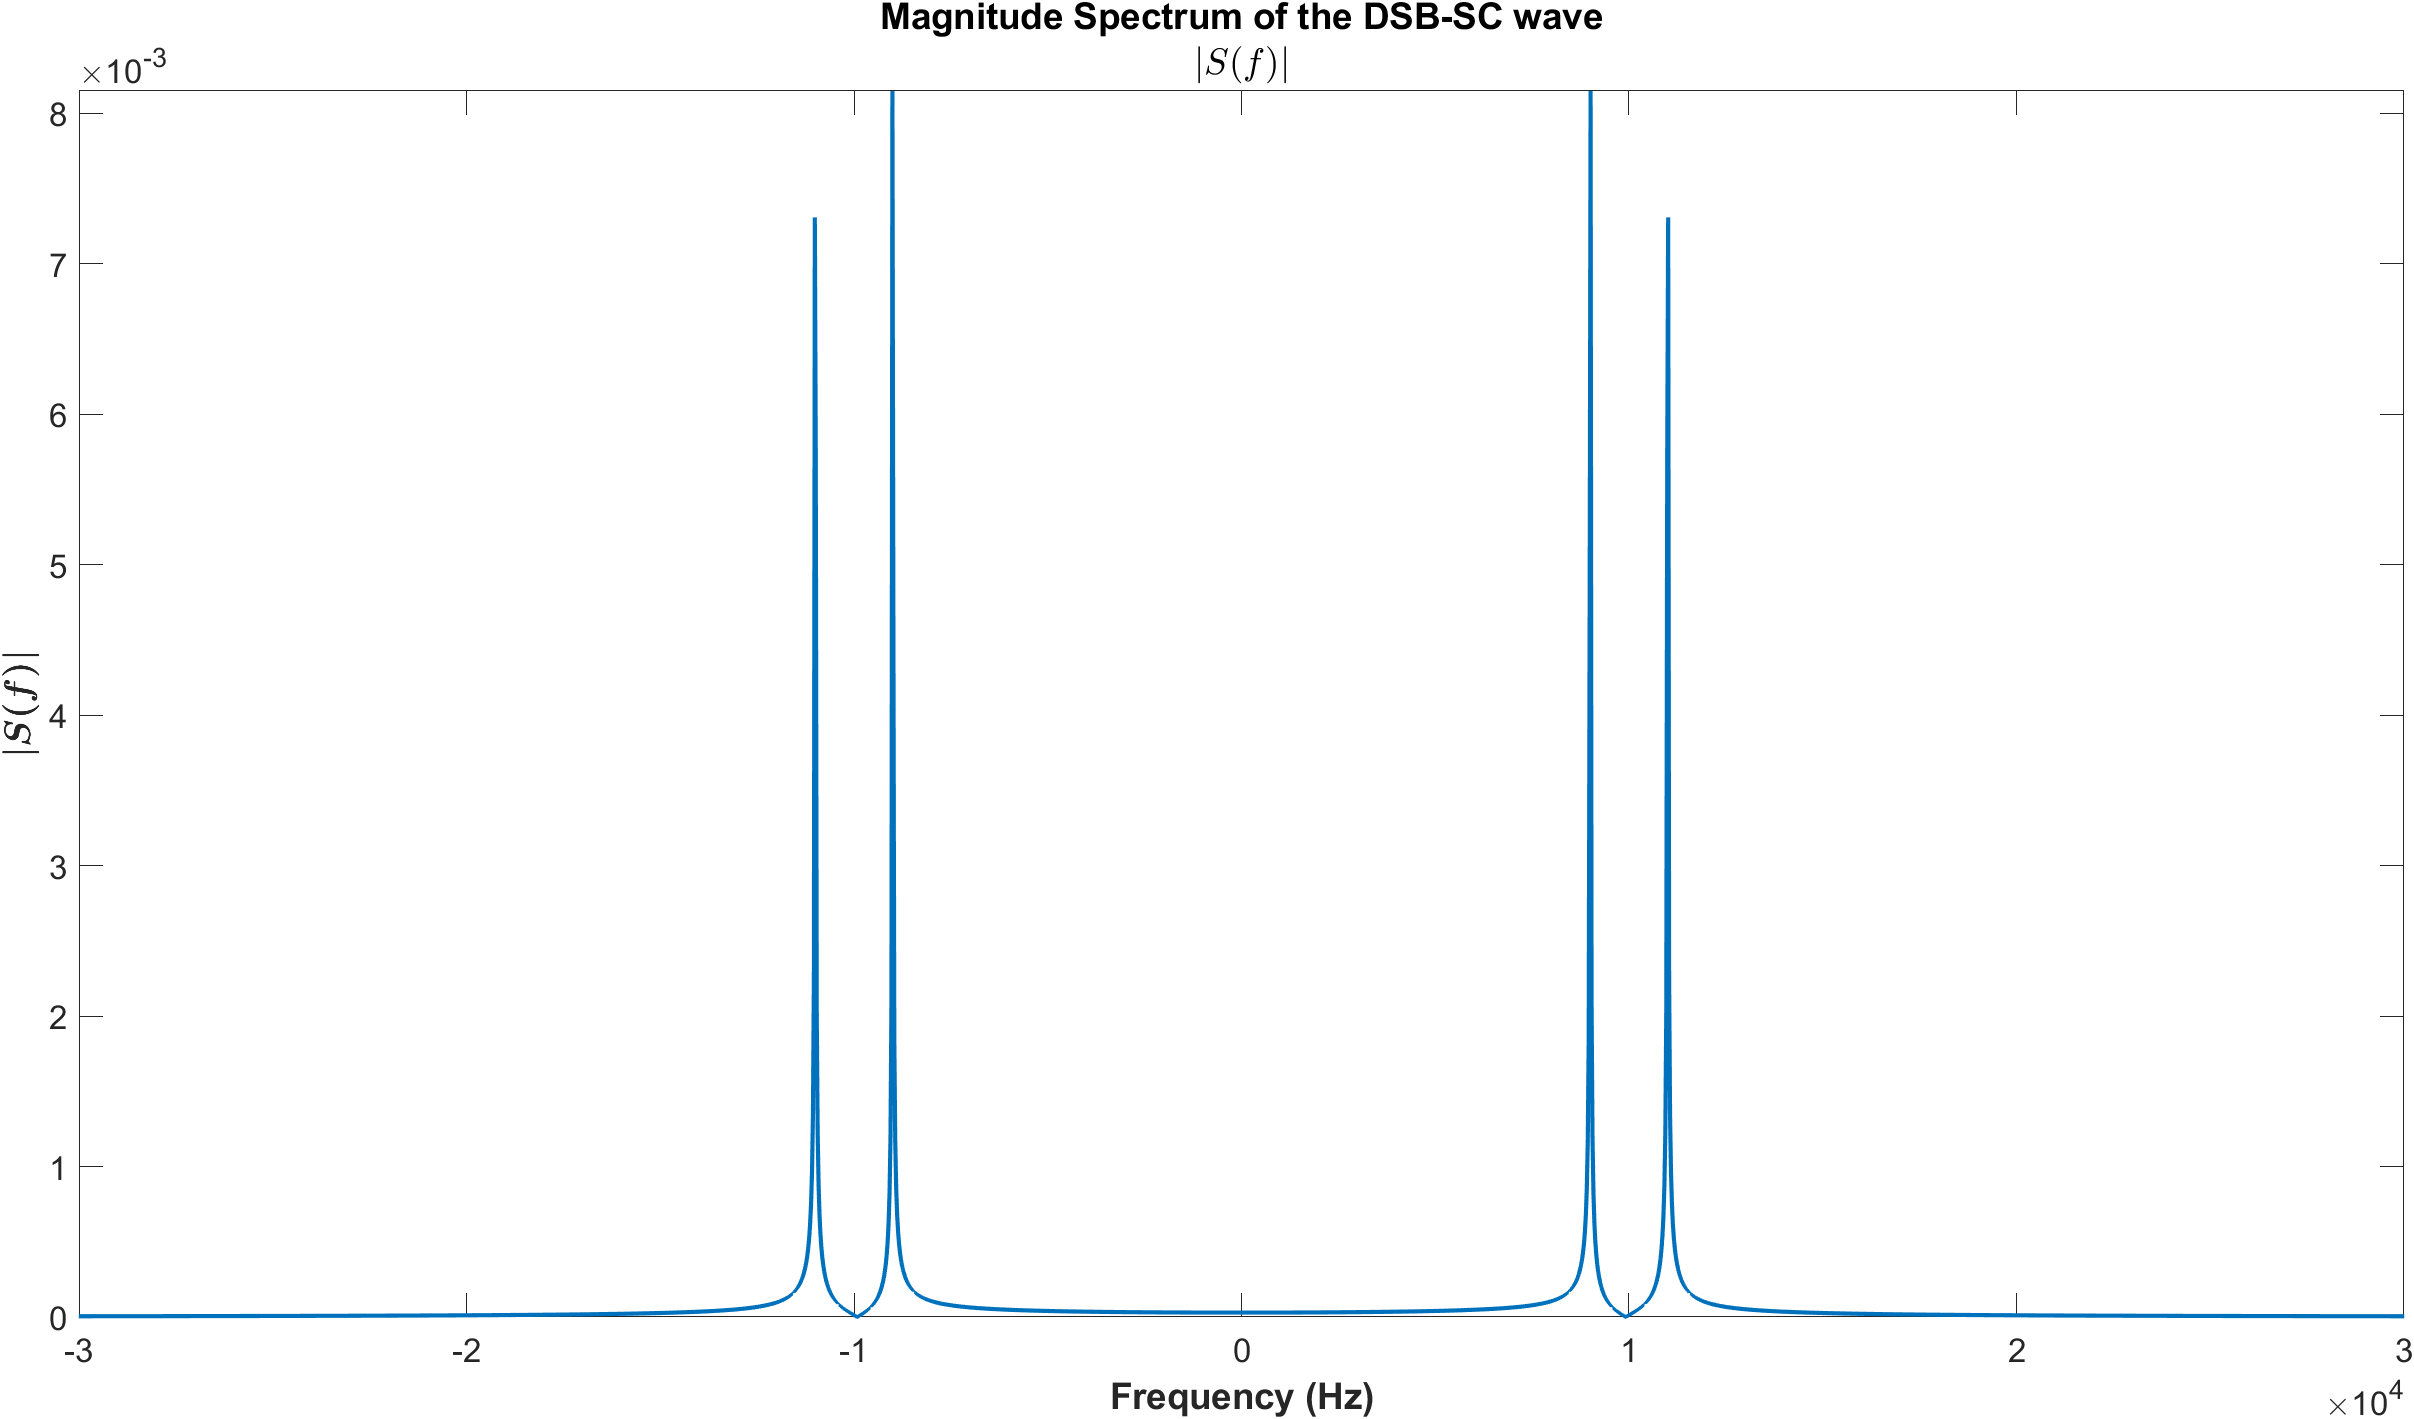
\includegraphics[width=\textwidth]{dsbsc_freq}
    \caption{\label{fig:dsbsc_freq}The Magnitude Spectrum of the DSB-SC Signal}
\end{figure} \clearpage

The remodulated DSB-SC signal $\hat{s}(t)$ is plotted in the time domain in Figure~\ref{fig:dsbsc_remod_time} and plotted in the frequency domain (magnitude spectrum) in Figure~\ref{fig:dsbsc_remod_freq}. The remodulated DSB-SC signal $\hat{s}(t)$ is found by multiplying $s(t)$ by the local carrier $\cos(2 \pi f_c t + \theta)$, when $\theta = 0$. A portion of the MATLAB code used to generate the remodulated DSB-SC signal is shown in Listing~\ref{listing:dsbsc_remod}.

\lstinputlisting[style=Matlab-editor, caption={Generating the Remodulated DSB-SC Signal}, label={listing:dsbsc_remod}, linerange={64-67}]{exp3_1.m}

\begin{figure}[h]
    \centering
    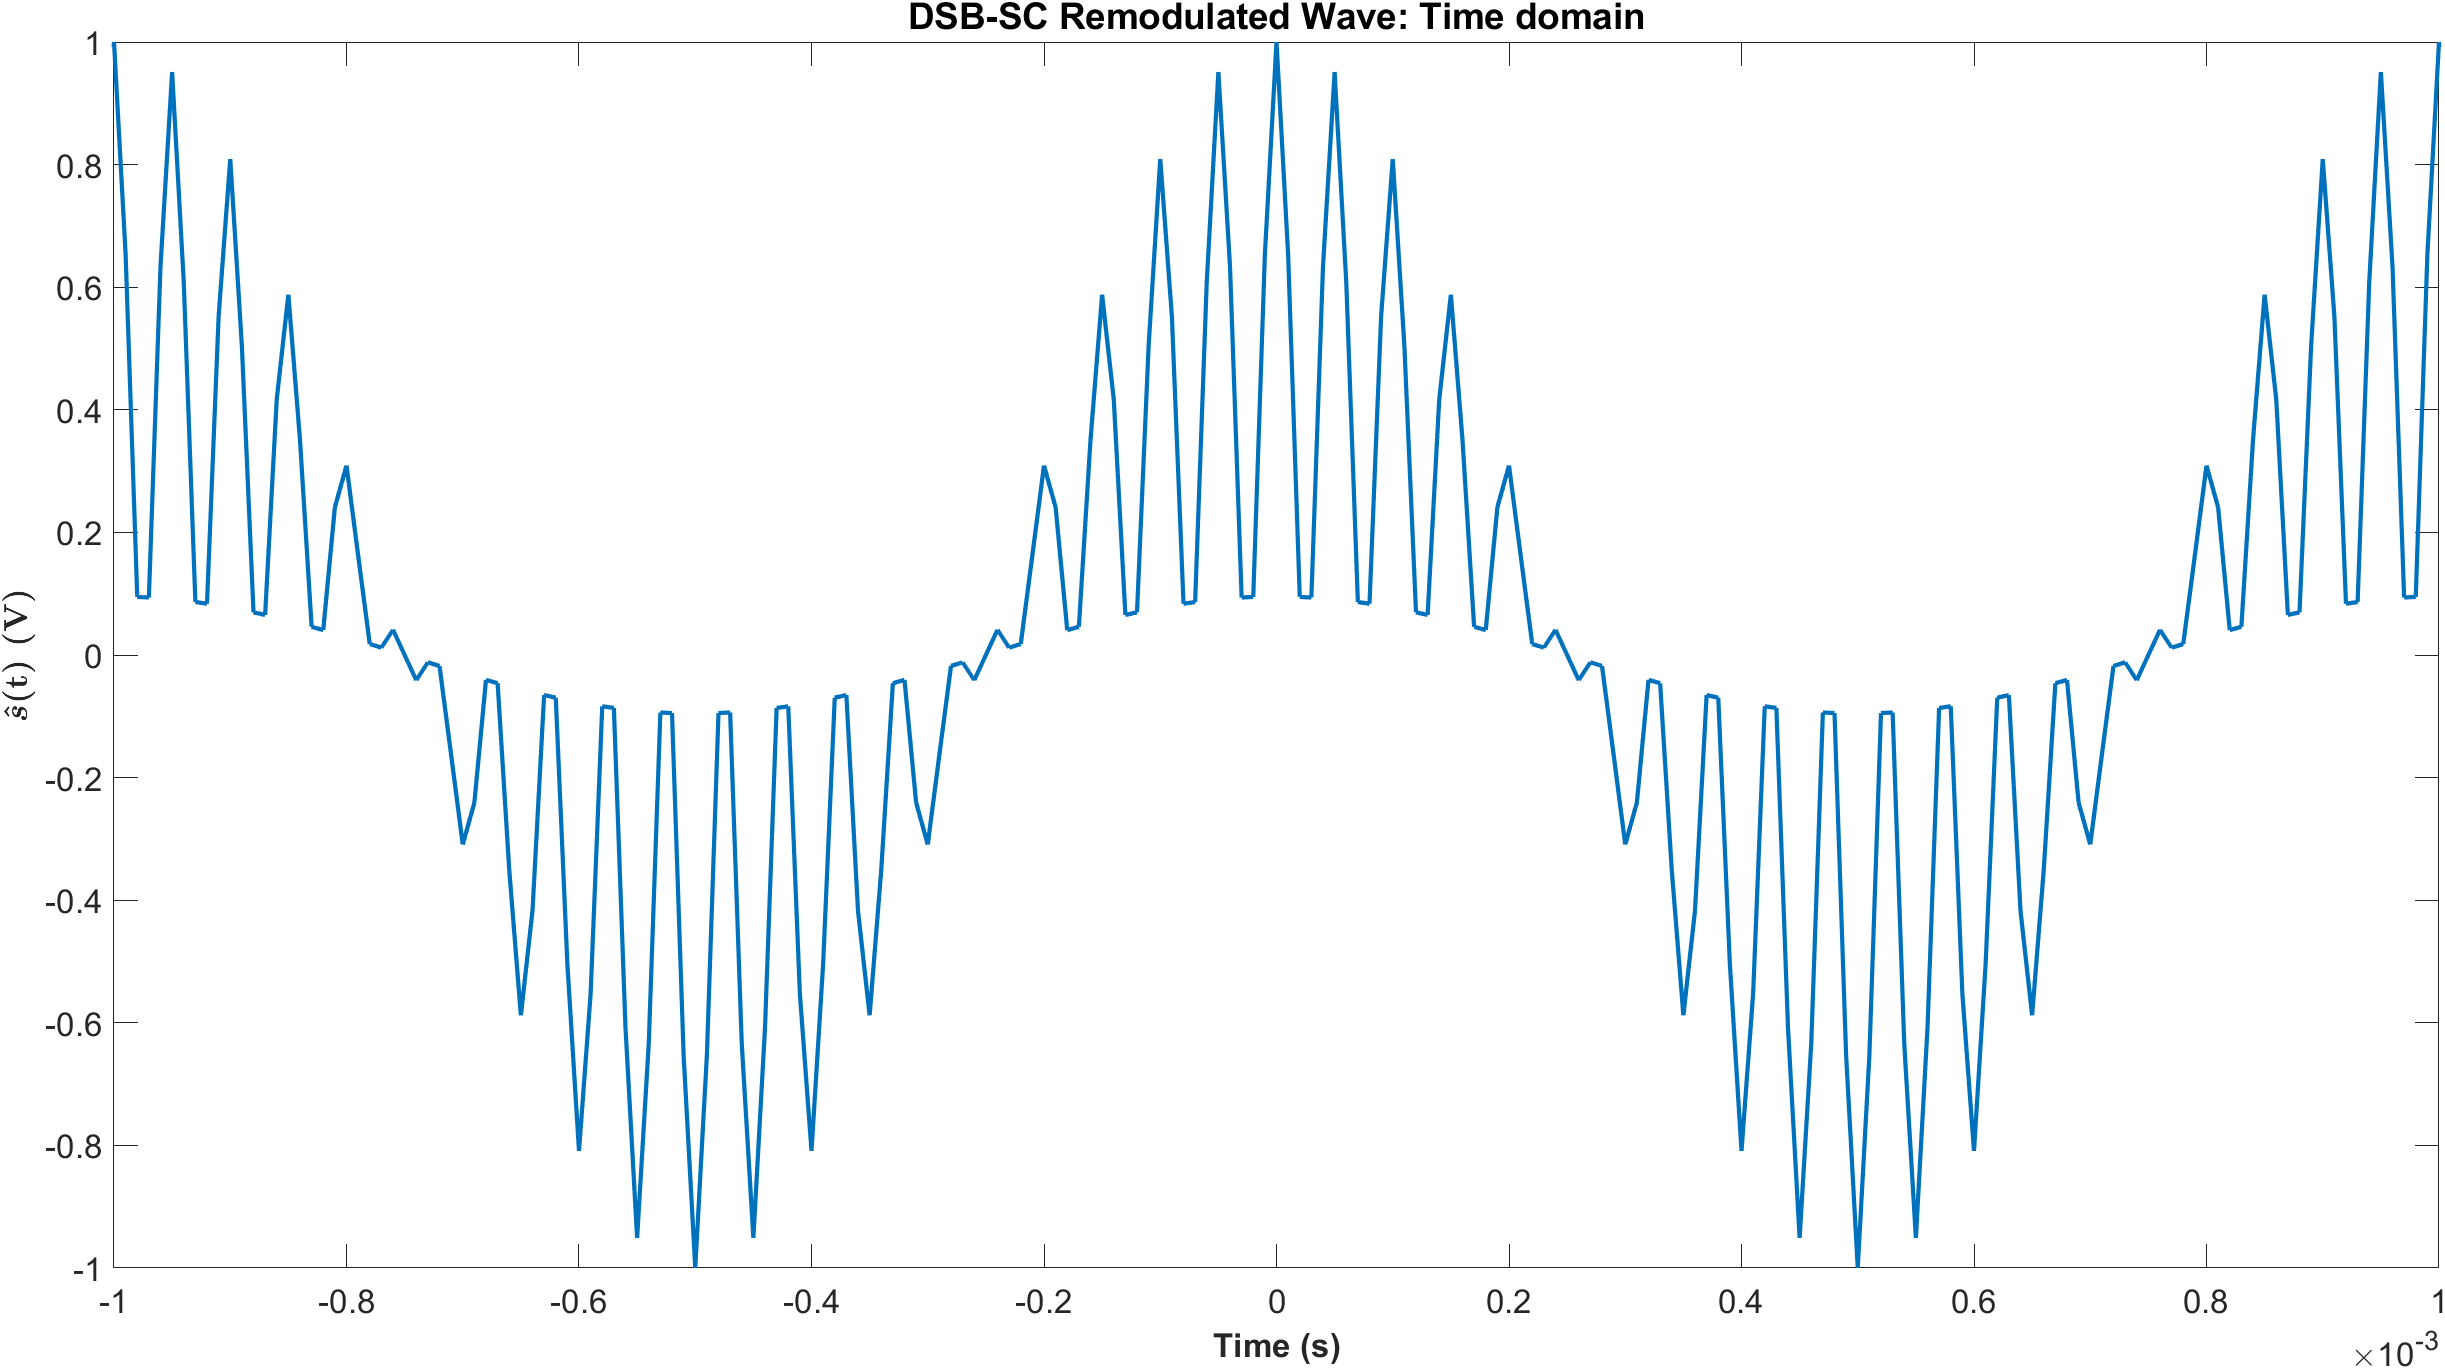
\includegraphics[width=0.76\textwidth]{dsbsc_remod_time}
    \caption{\label{fig:dsbsc_remod_time}The Remodulated DSB-SC Signal in Time Domain}
\end{figure}
\begin{figure}[h]
    \centering
    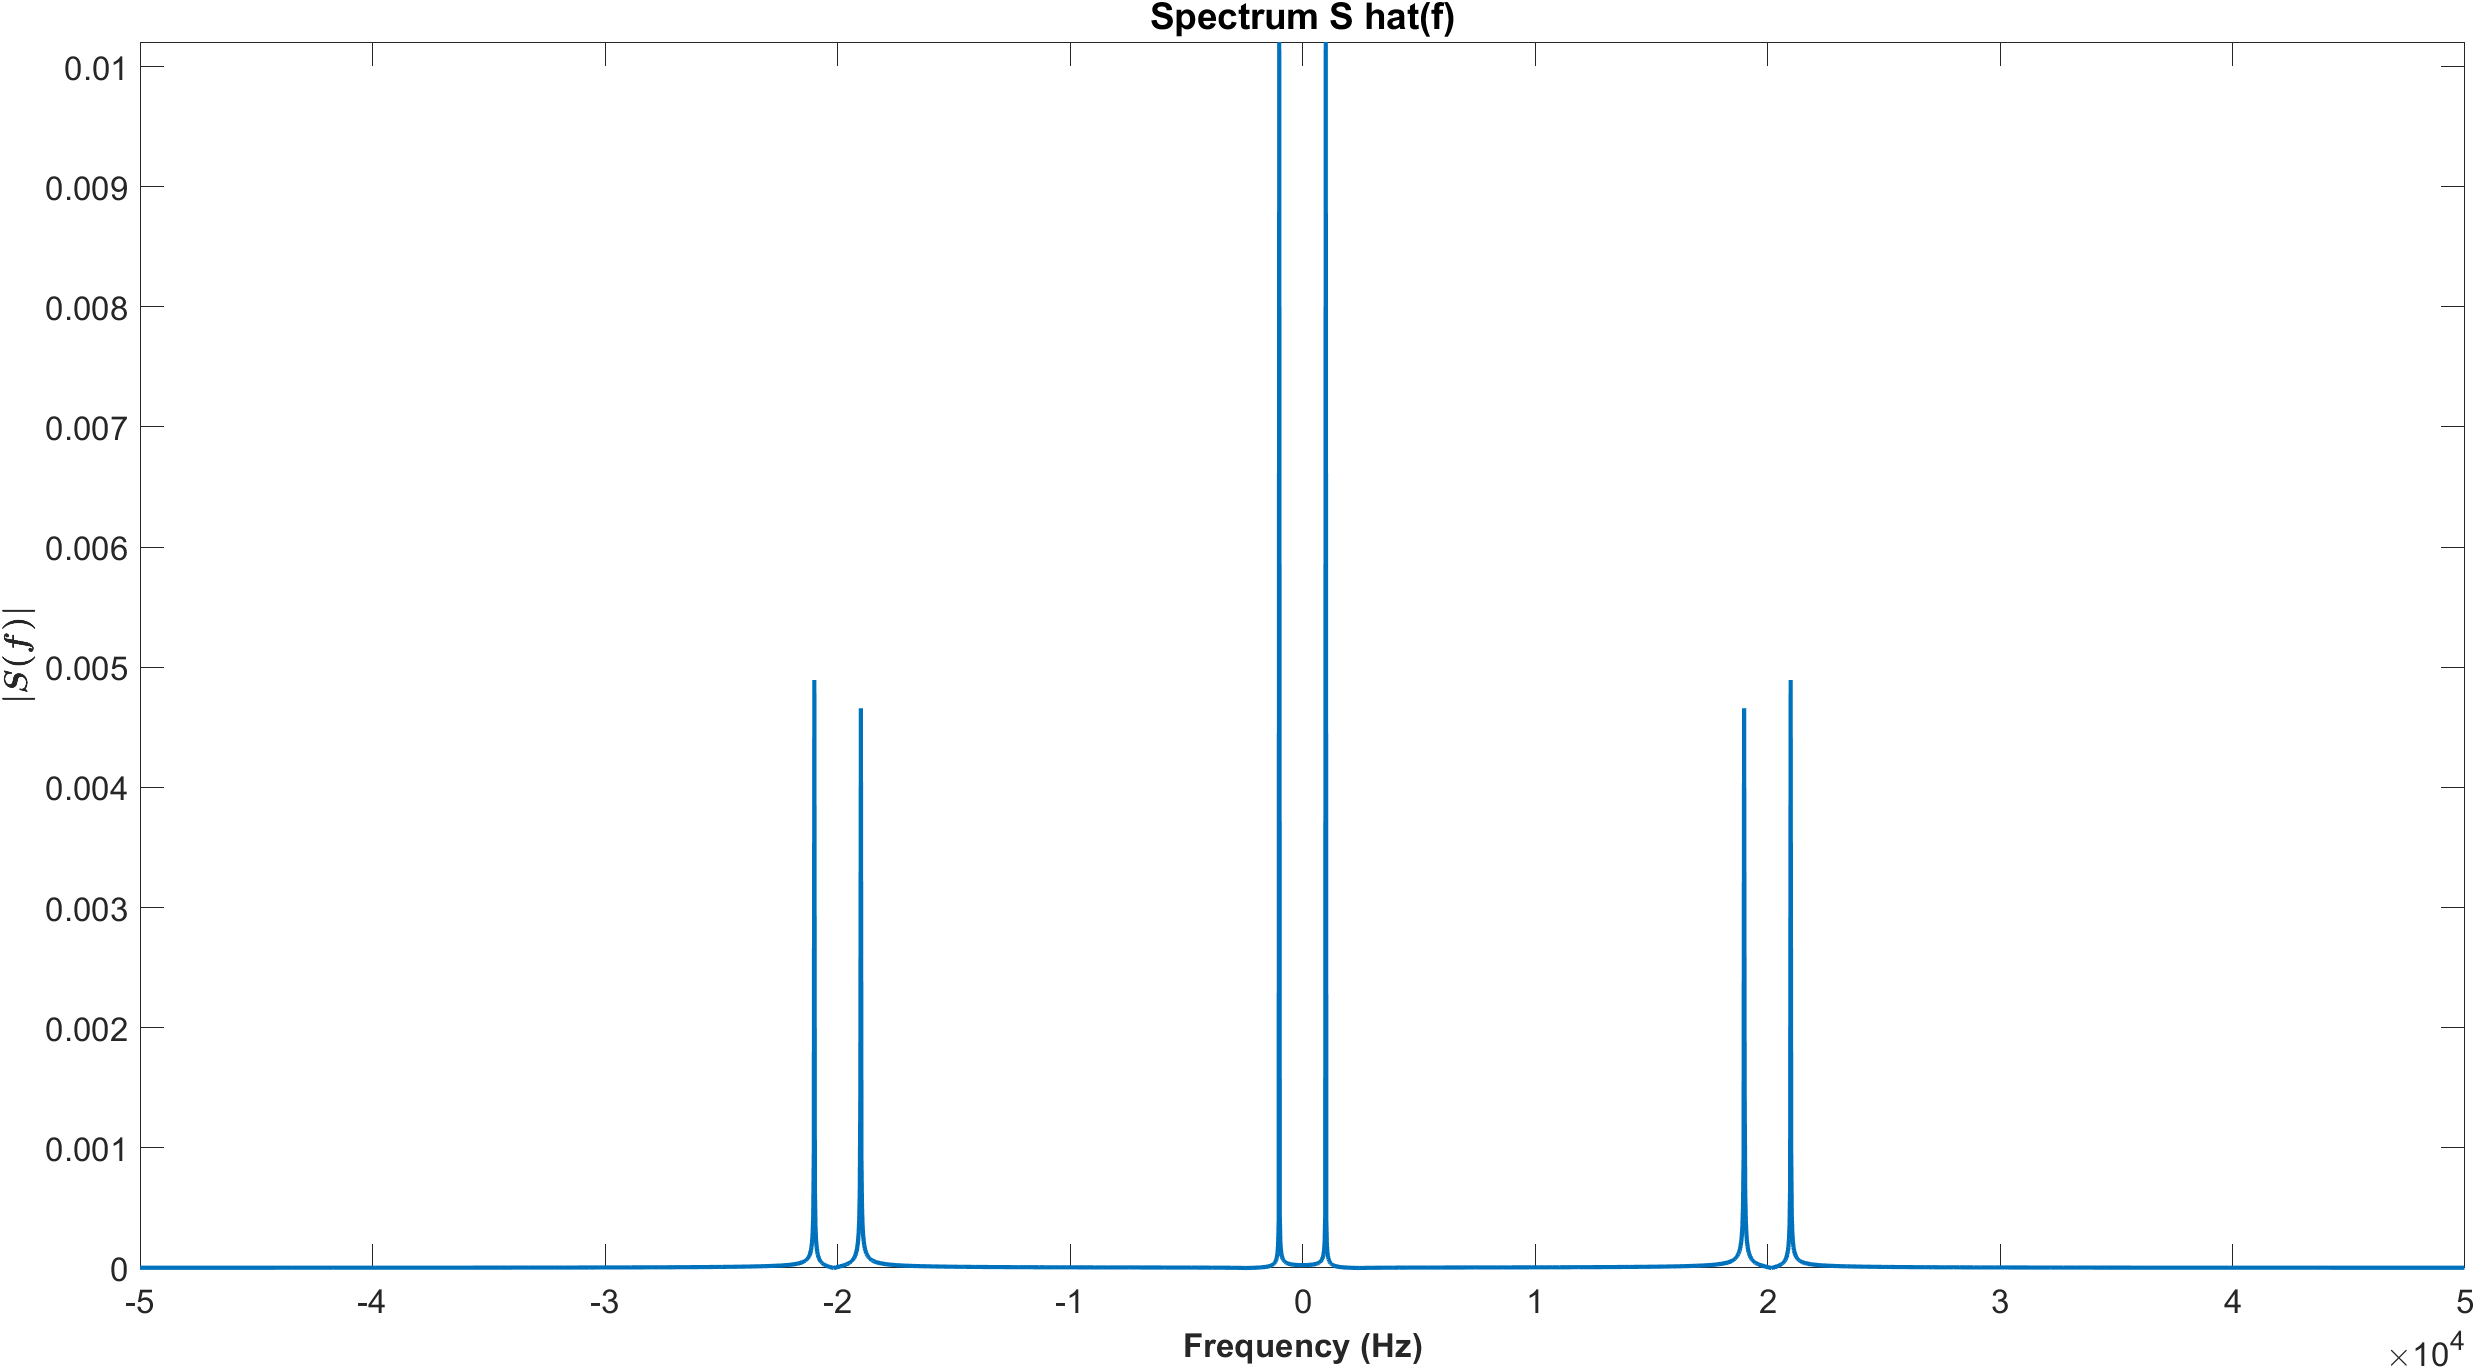
\includegraphics[width=0.76\textwidth]{dsbsc_remod_freq}
    \caption{\label{fig:dsbsc_remod_freq}The Magnitude Spectrum of the Remodulated DSB-SC Signal}
\end{figure} \clearpage

The original message signal $m(t)$ can be retrieved from the remodulated DSB-SC signal $\hat{s}(t)$ by passing $\hat{s}(t)$ through a low-pass filter. The output of the filtered remodulated DSB-SC signal at $\theta$ values of $0$, $\pi/2$, and $\pi/4$ are shown in Figures \ref{fig:dsbsc_lpf_0}, \ref{fig:dsbsc_lpf_p2}, and \ref{fig:dsbsc_lpf_p4}. The MATLAB function to plot the output of the low-pass filter is shown in Listing~\ref{listing:dsbsc_lpf}.

\lstinputlisting[style=Matlab-editor, caption={Plotting the Output of the Low-pass Filter}, label={listing:dsbsc_lpf}, linerange={116-145}]{exp3_1.m}

\begin{figure}[h]
    \centering
    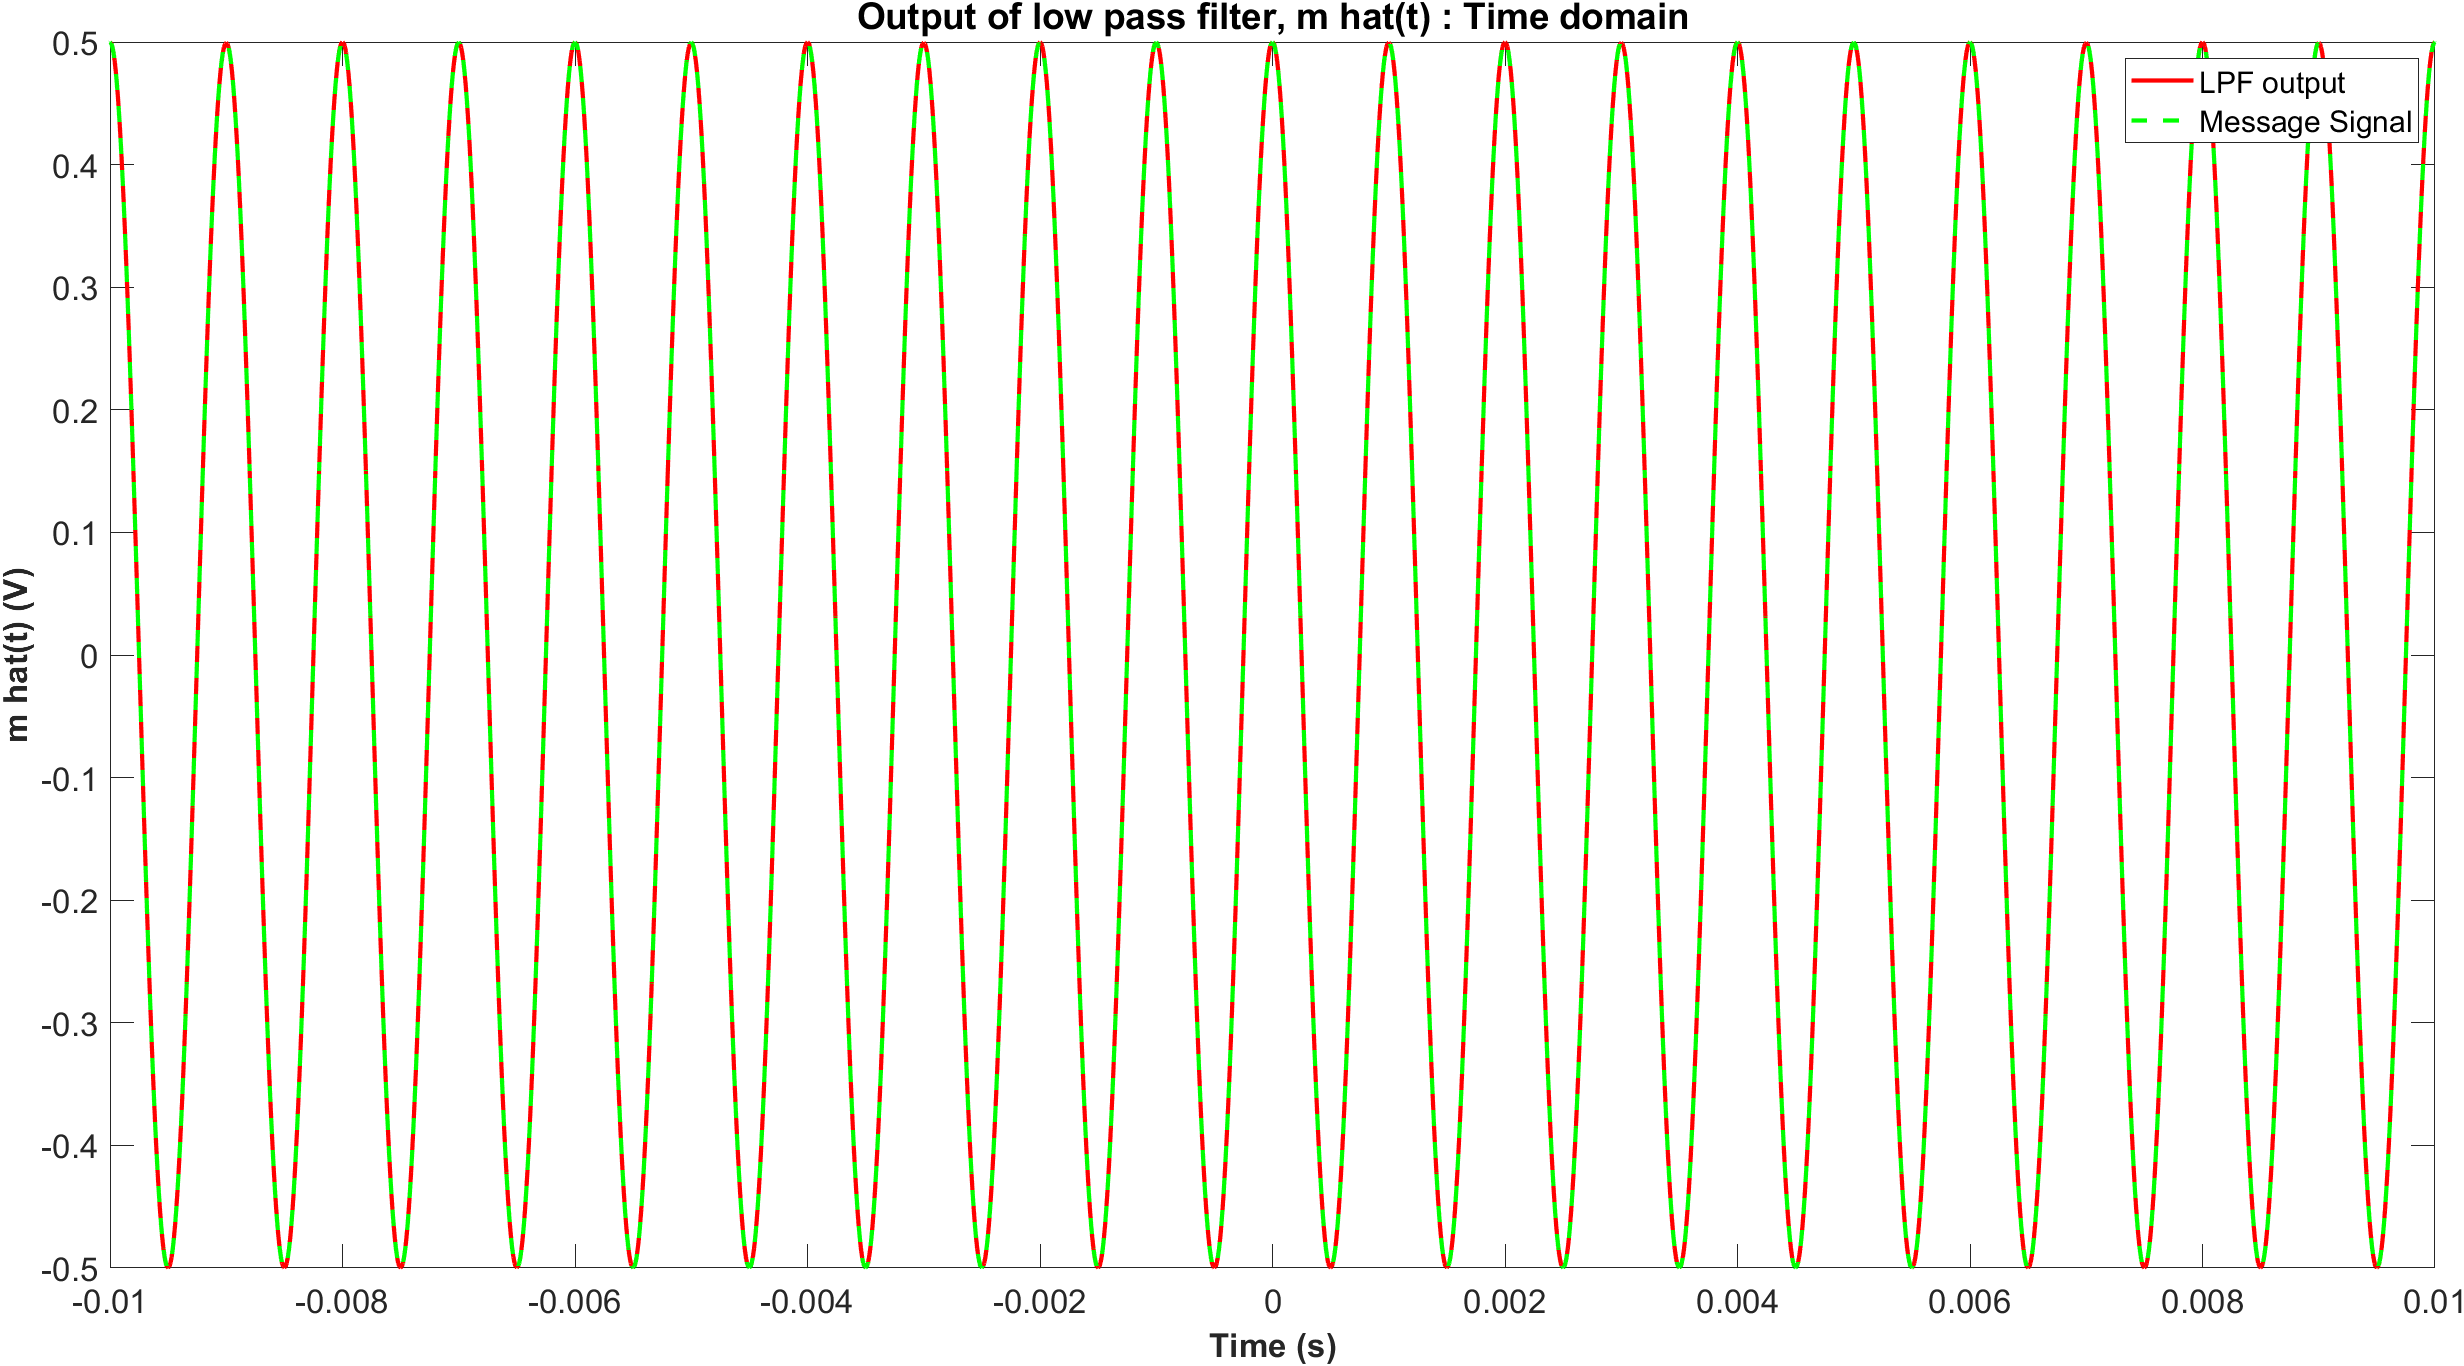
\includegraphics[width=0.68\textwidth]{dsbsc_remod_lpf_theta_0}
    \caption{\label{fig:dsbsc_lpf_0}The Low-pass Filter Output for $\theta = 0$}
\end{figure}
\begin{figure}[h]
    \centering
    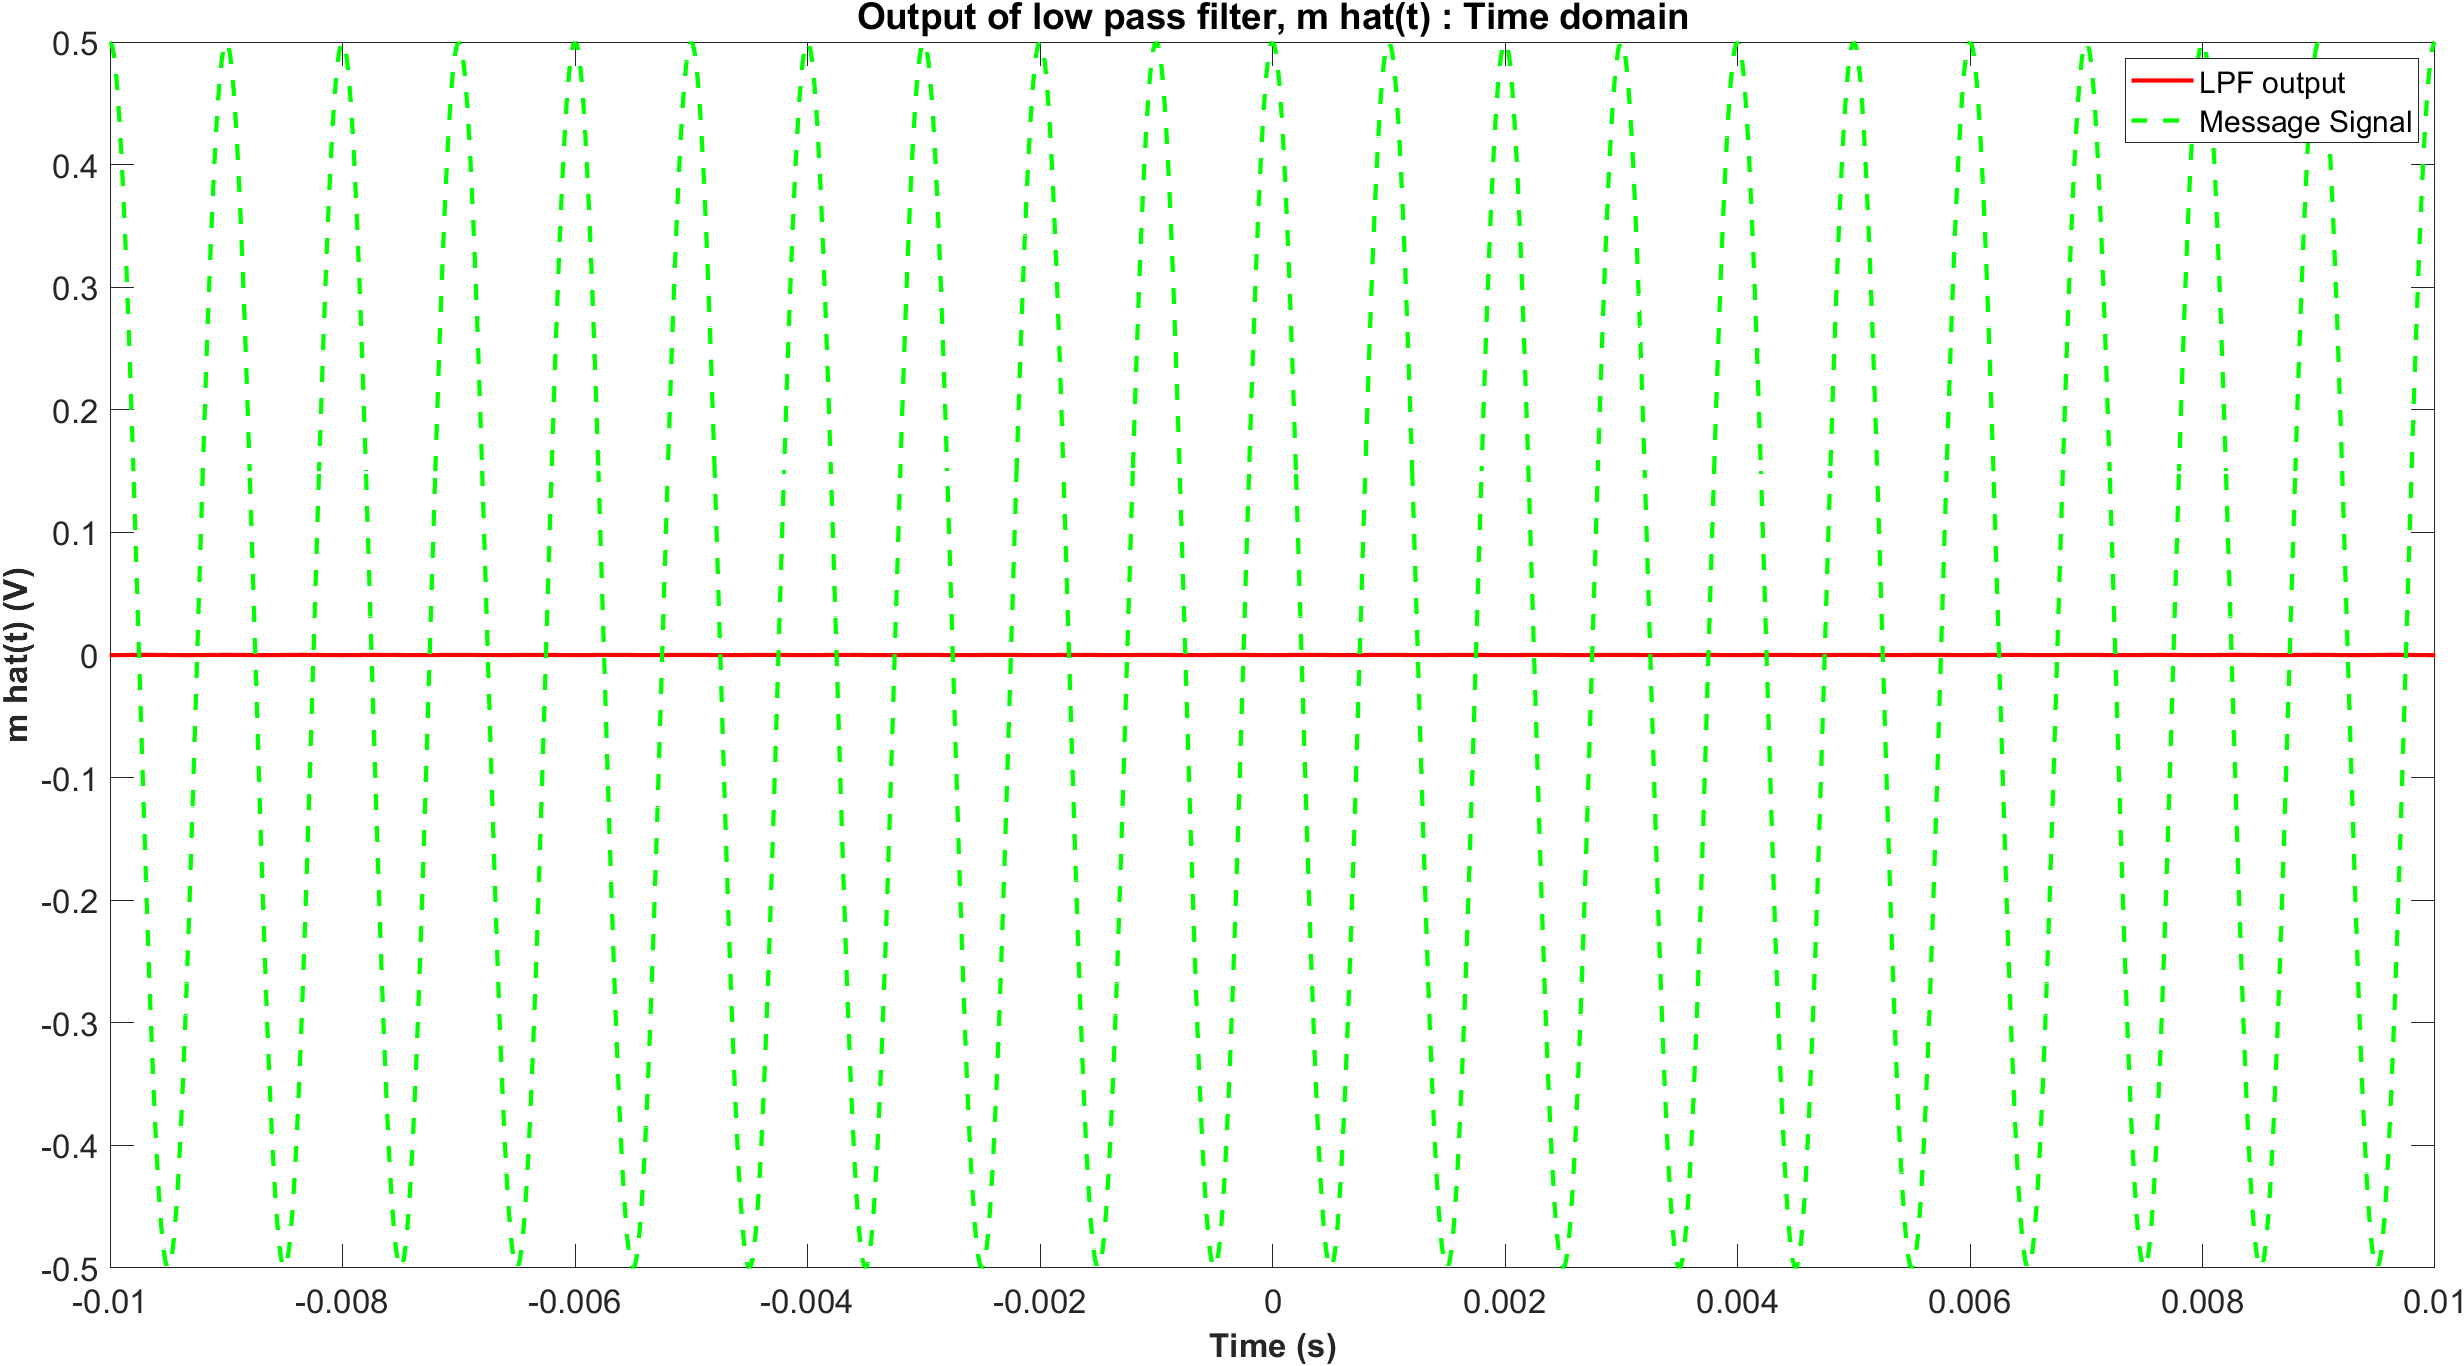
\includegraphics[width=0.68\textwidth]{dsbsc_remod_lpf_theta_1.5708}
    \caption{\label{fig:dsbsc_lpf_p2}The Low-pass Filter Output for $\theta = \pi/2$}
\end{figure}
\begin{figure}[h]
    \centering
    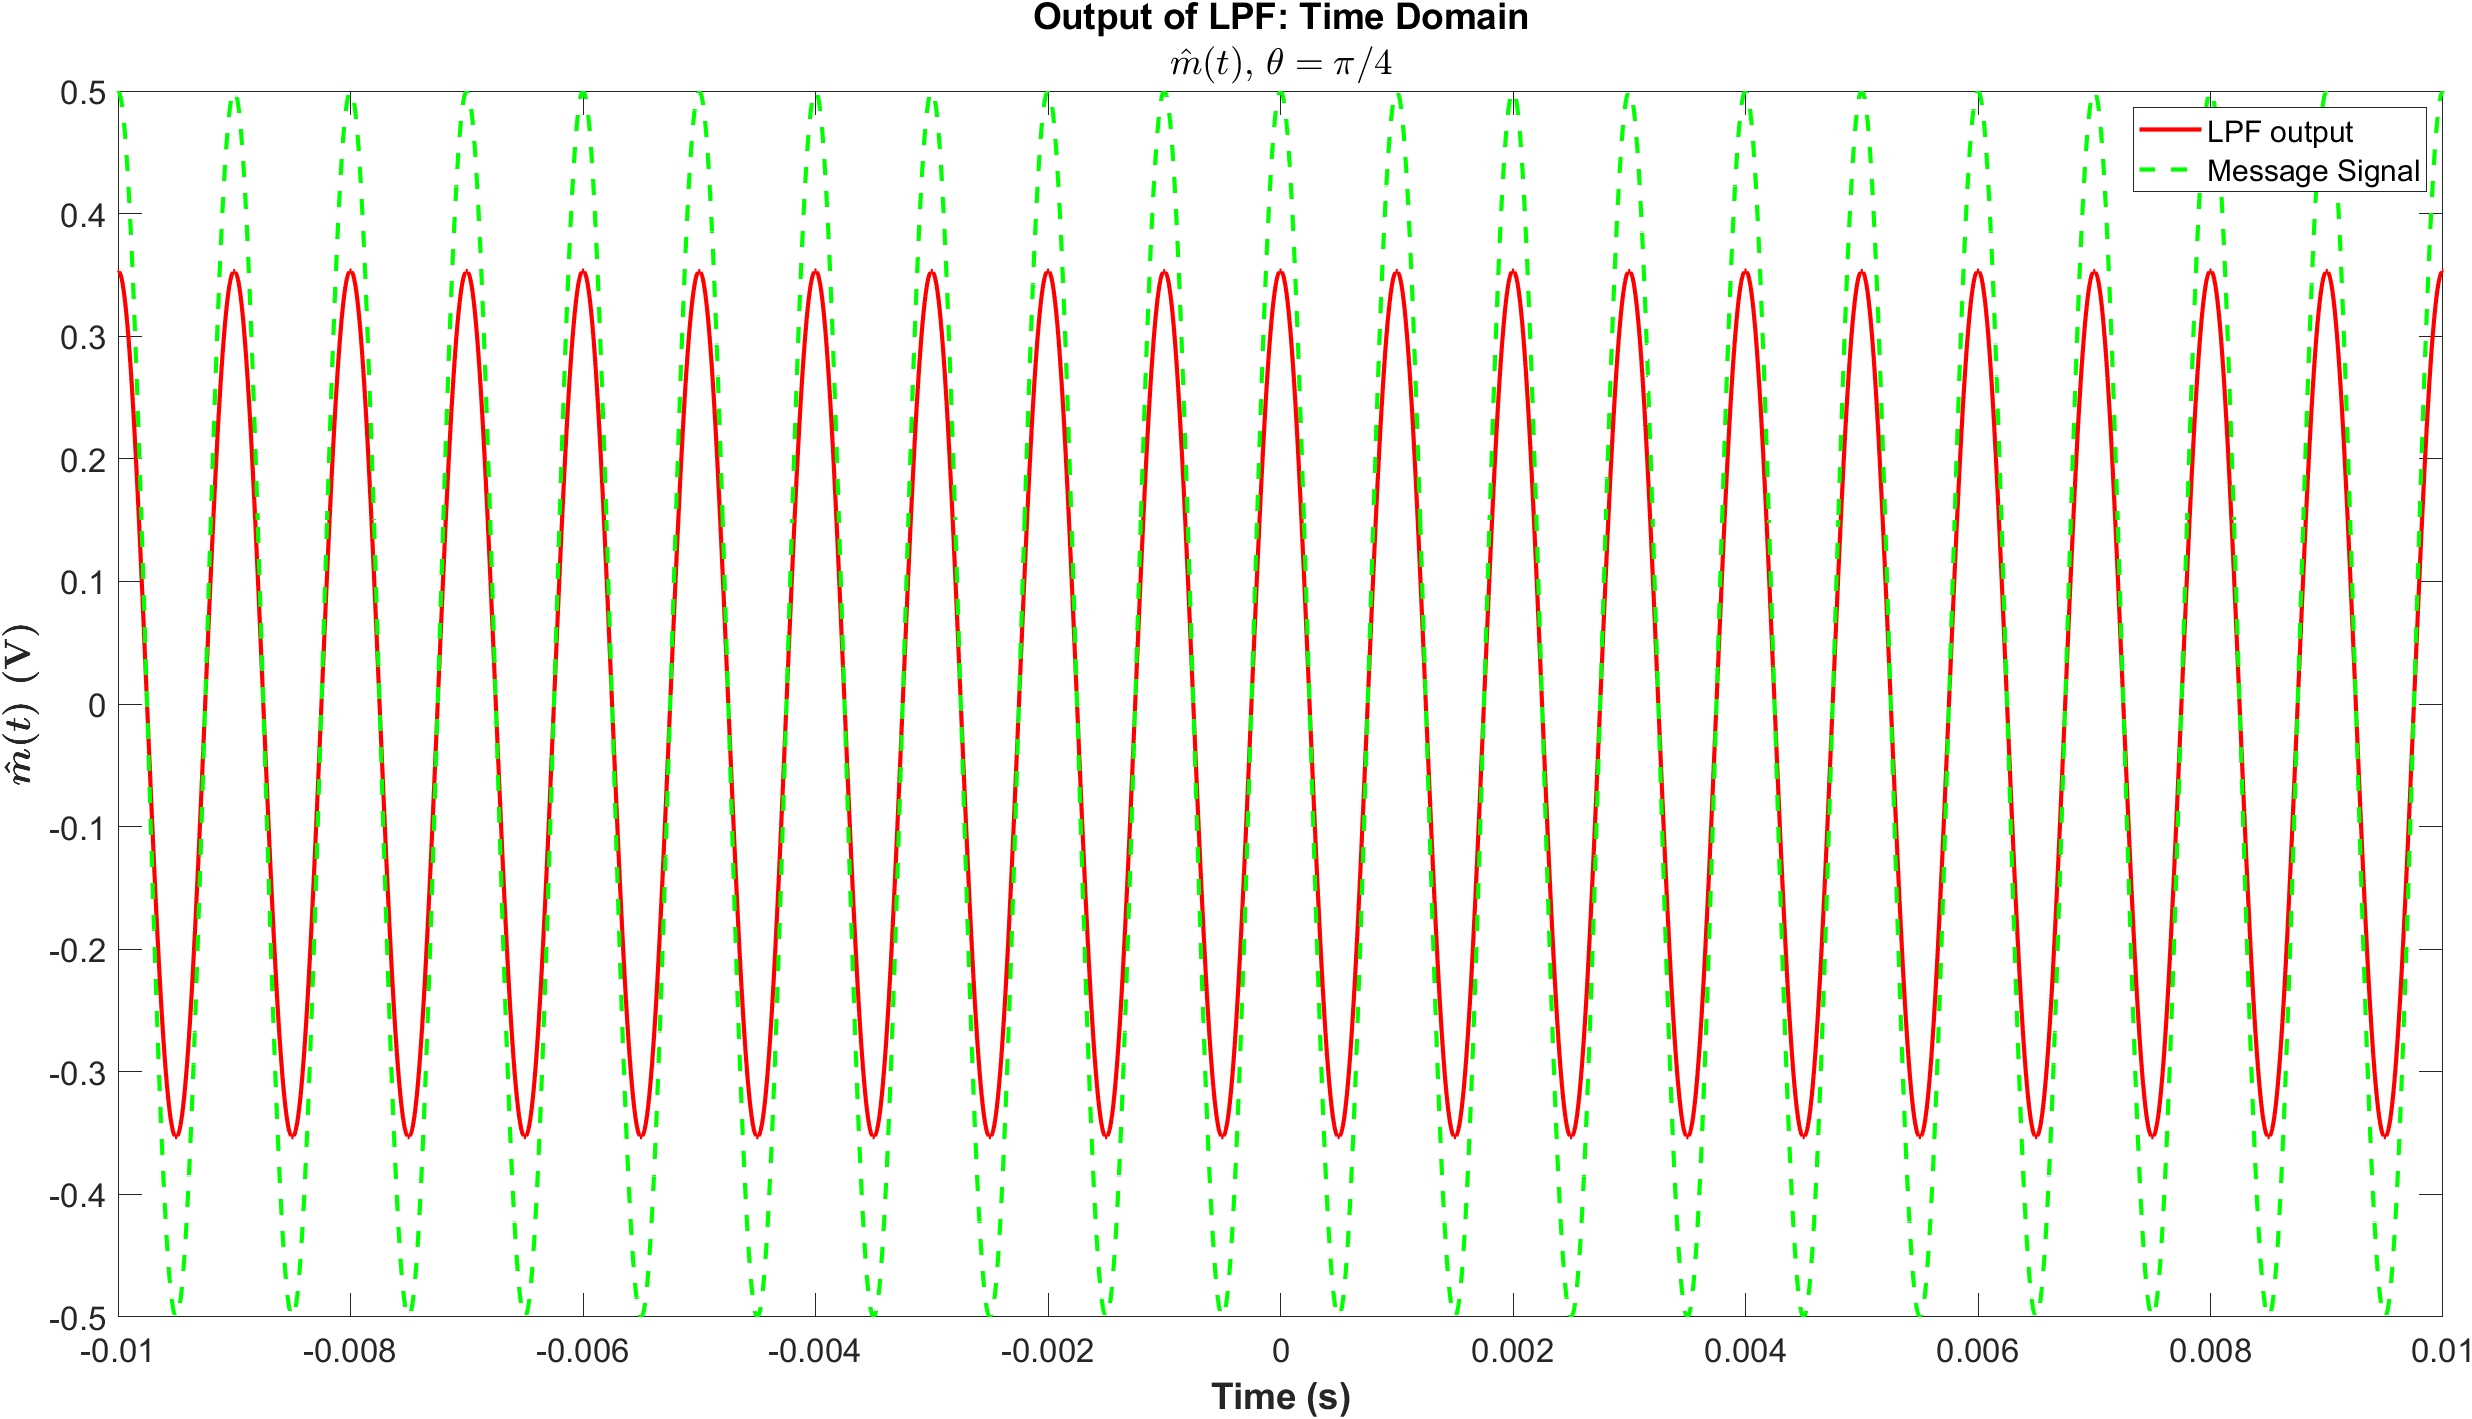
\includegraphics[width=0.68\textwidth]{dsbsc_remod_lpf_theta_0.7854}
    \caption{\label{fig:dsbsc_lpf_p4}The Low-pass Filter Output for $\theta = \pi/4$}
\end{figure} \clearpage

The low-pass filter used for all three signals is an ideal low-pass filter with a cut-off frequency of 1.5 kHz. The possible ranges for the cut-off frequency of the low-pass filter depends on the message frequency $f_m$, and the carrier frequency, $f_c$. We can see from Figure~\ref{fig:dsbsc_remod_freq} that there are impulses at $\pm 1$ kHz ($\pm f_m$), and impulses are $\pm 19$ and $\pm 21$ kHz ($\pm 2f_c \pm f_m$). We want the low-pass filter to filter frequency components around the impulses at $\pm f_m$, without attenuating the frequency components around $\pm 2f_c \pm f_m$. Therefore the possible range of cut-off frequencies range from slightly above 1 kHz (around 1.3 kHz) to slightly below 19 kHz (around 17.5 kHz).

We can see that when $\theta = 0$, we retrieve the message signal perfectly with no attenuation, while when $\theta = \pi/4$, the message signal is attenuated but can still be retrieved after amplification. In the case where $\theta = \pi/2$, we see that there is no signal at the output of the low-pass filter. This corresponds to the quadrature null effect, where the phase difference between the local oscillator and the carrier signal can lead to the amplitude of the demodulated signal to equal zero. This illustrates the need for phase synchronization, as without ensuring that the local oscillator and the carrier signal are in-phase we may lose some of the signal strength of the original message signal, or lose the signal entirely in the case of the quadrature null effect.

\section*{Numerical Experiment 3.2: QAM Signal}
The first message signal is given by Equation~\ref{eq:qam_m1}, and the second message signal is given by Equation~\ref{eq:qam_m2} where $T_m = 0.001$ s.
\begin{gather}
    m_1(t) = 2 \sinc{\left(t / T_m\right)} \label{eq:qam_m1} \\
    m_2(t) = \sinc^2{\left(t / T_m\right)} \label{eq:qam_m2}
\end{gather}
The QAM signal is given by Equation~\ref{eq:qam}, where $A_c$ = 1 V, and $f_c$ = 10 kHz.
\begin{equation} \label{eq:qam}
    s(t) = A_c \left[ m_1(t) \cos(2 \pi f_c t) + m_2(t) \sin(2 \pi f_c t) \right]    
\end{equation}

The QAM signal is plotted in the time domain in Figure~\ref{fig:qam_time} and plotted in the frequency domain (magnitude spectrum) in Figure~\ref{fig:qam_freq}. A portion of the MATLAB code used to generate the QAM signal is shown in Listing~\ref{listing:qam}.

\lstinputlisting[style=Matlab-editor, caption={Generating the QAM Signal}, label={listing:qam}, linerange={18-33}]{exp3_2.m}

\begin{figure}[h]
    \centering
    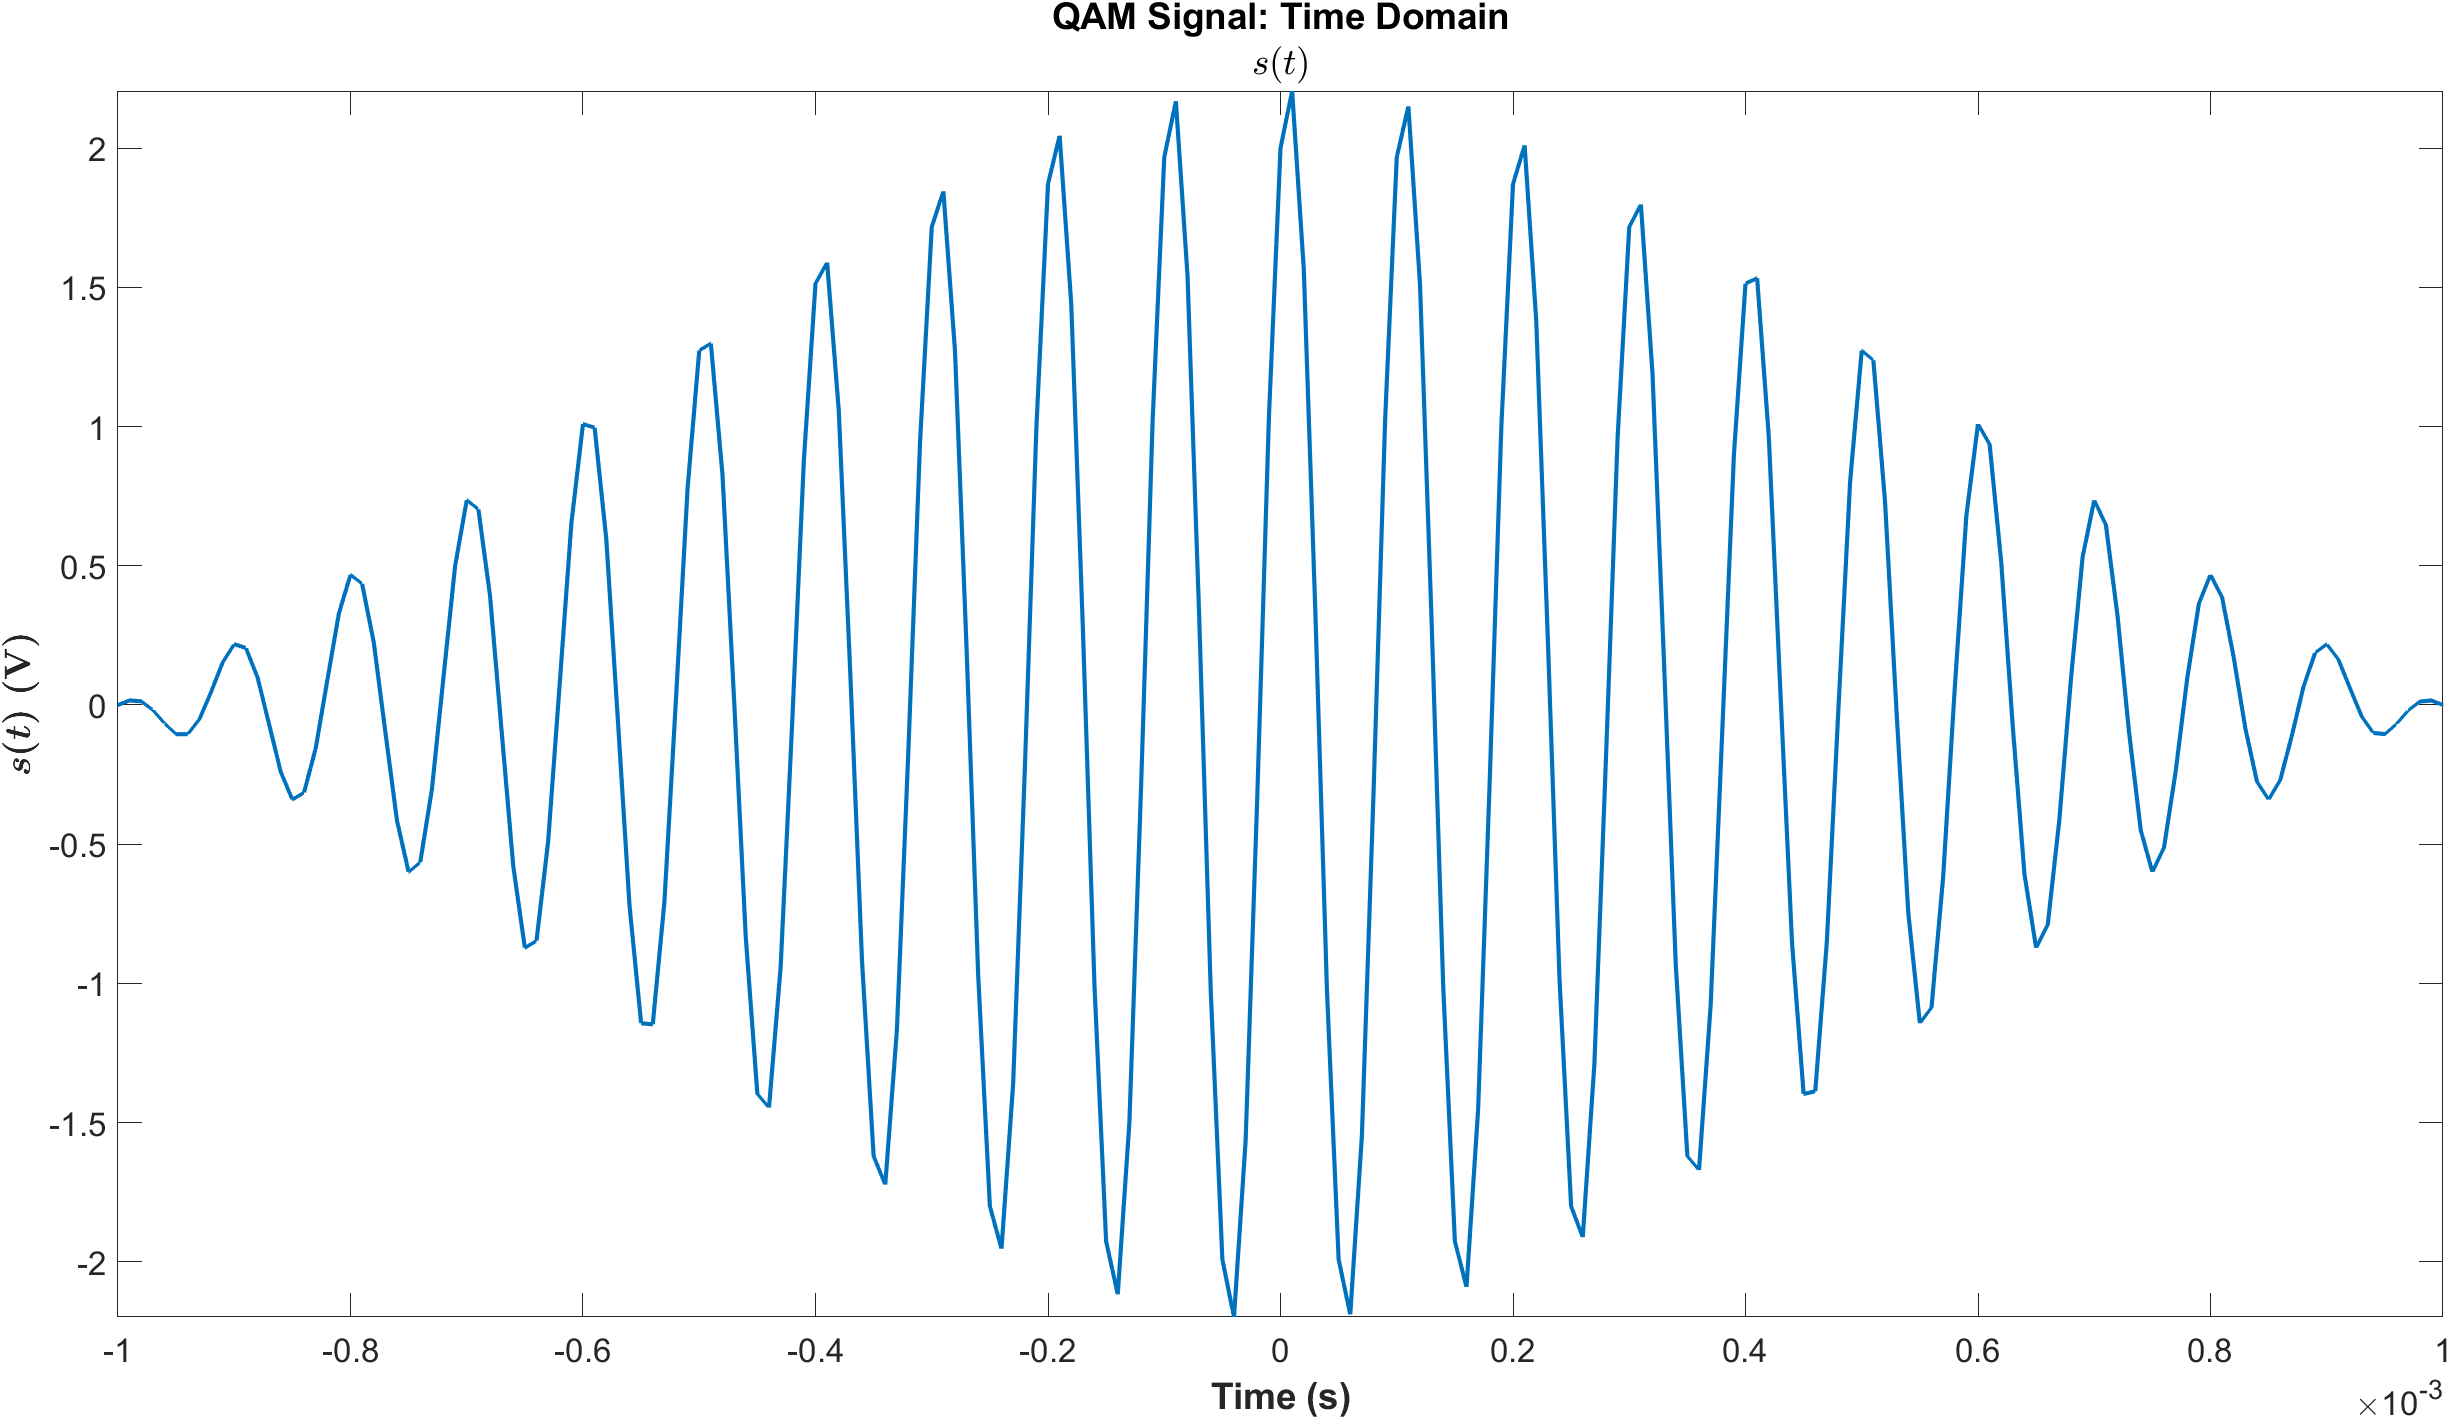
\includegraphics[width=0.78\textwidth]{qam_time}
    \caption{\label{fig:qam_time}The QAM Signal in Time Domain}
\end{figure}
\begin{figure}[h]
    \centering
    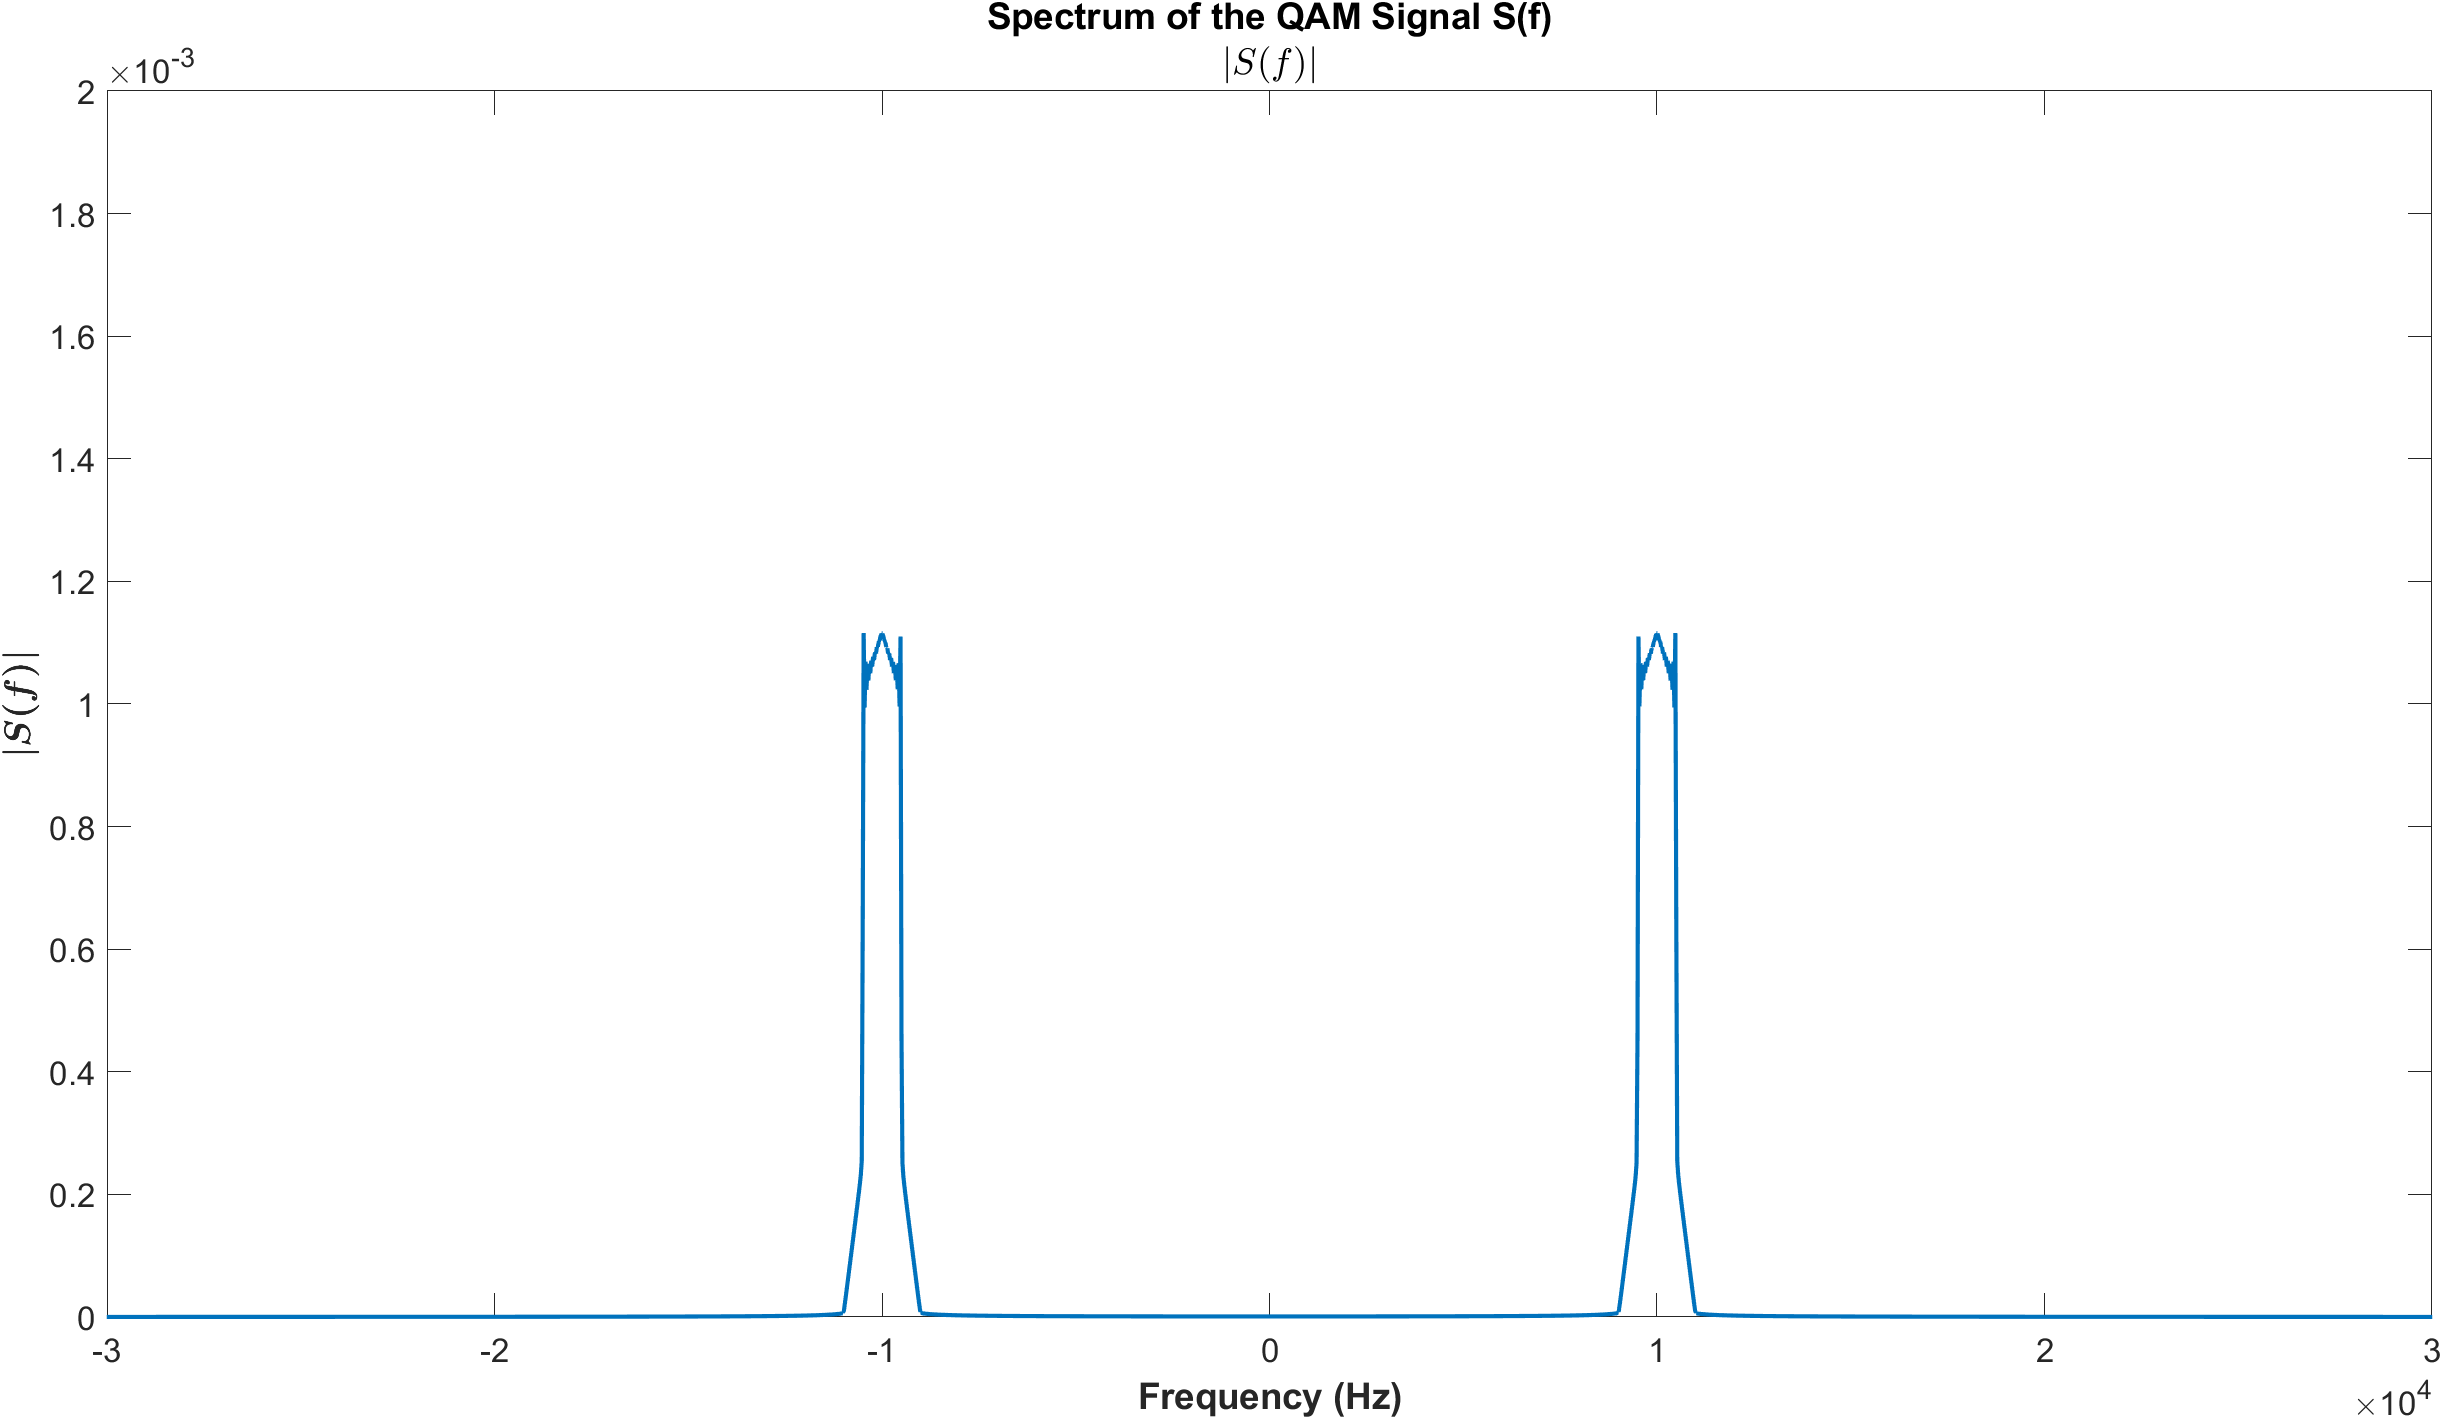
\includegraphics[width=0.78\textwidth]{qam_freq}
    \caption{\label{fig:qam_freq}The Magnitude Spectrum of the QAM Signal}
\end{figure} \clearpage

The QAM signal can be demodulated (in a similar fashion to the DSB-SC signal; multiplied by a local oscillator), and demultiplexed to retrieve the signals corresponding the in-phase and quadrature carriers. These signals can be passed through low-pass filters to retrieve the original message signal. The retrieved message signals when $\theta = 0$ and $\theta = \pi/4$ are shown in Figures \ref{fig:qam_demod_lpf_0} and \ref{fig:qam_demod_lpf_p4}. A portion of the MATLAB function to demodulated, demultiplex and retrieve the output of the low-pass filter is shown in Listing~\ref{listing:qam_lpf}.

\lstinputlisting[style=Matlab-editor, caption={Genearting the Output of the Low-pass Filter}, label={listing:qam_lpf}, linerange={72-97}]{exp3_2.m}

\begin{figure}[h]
    \centering
    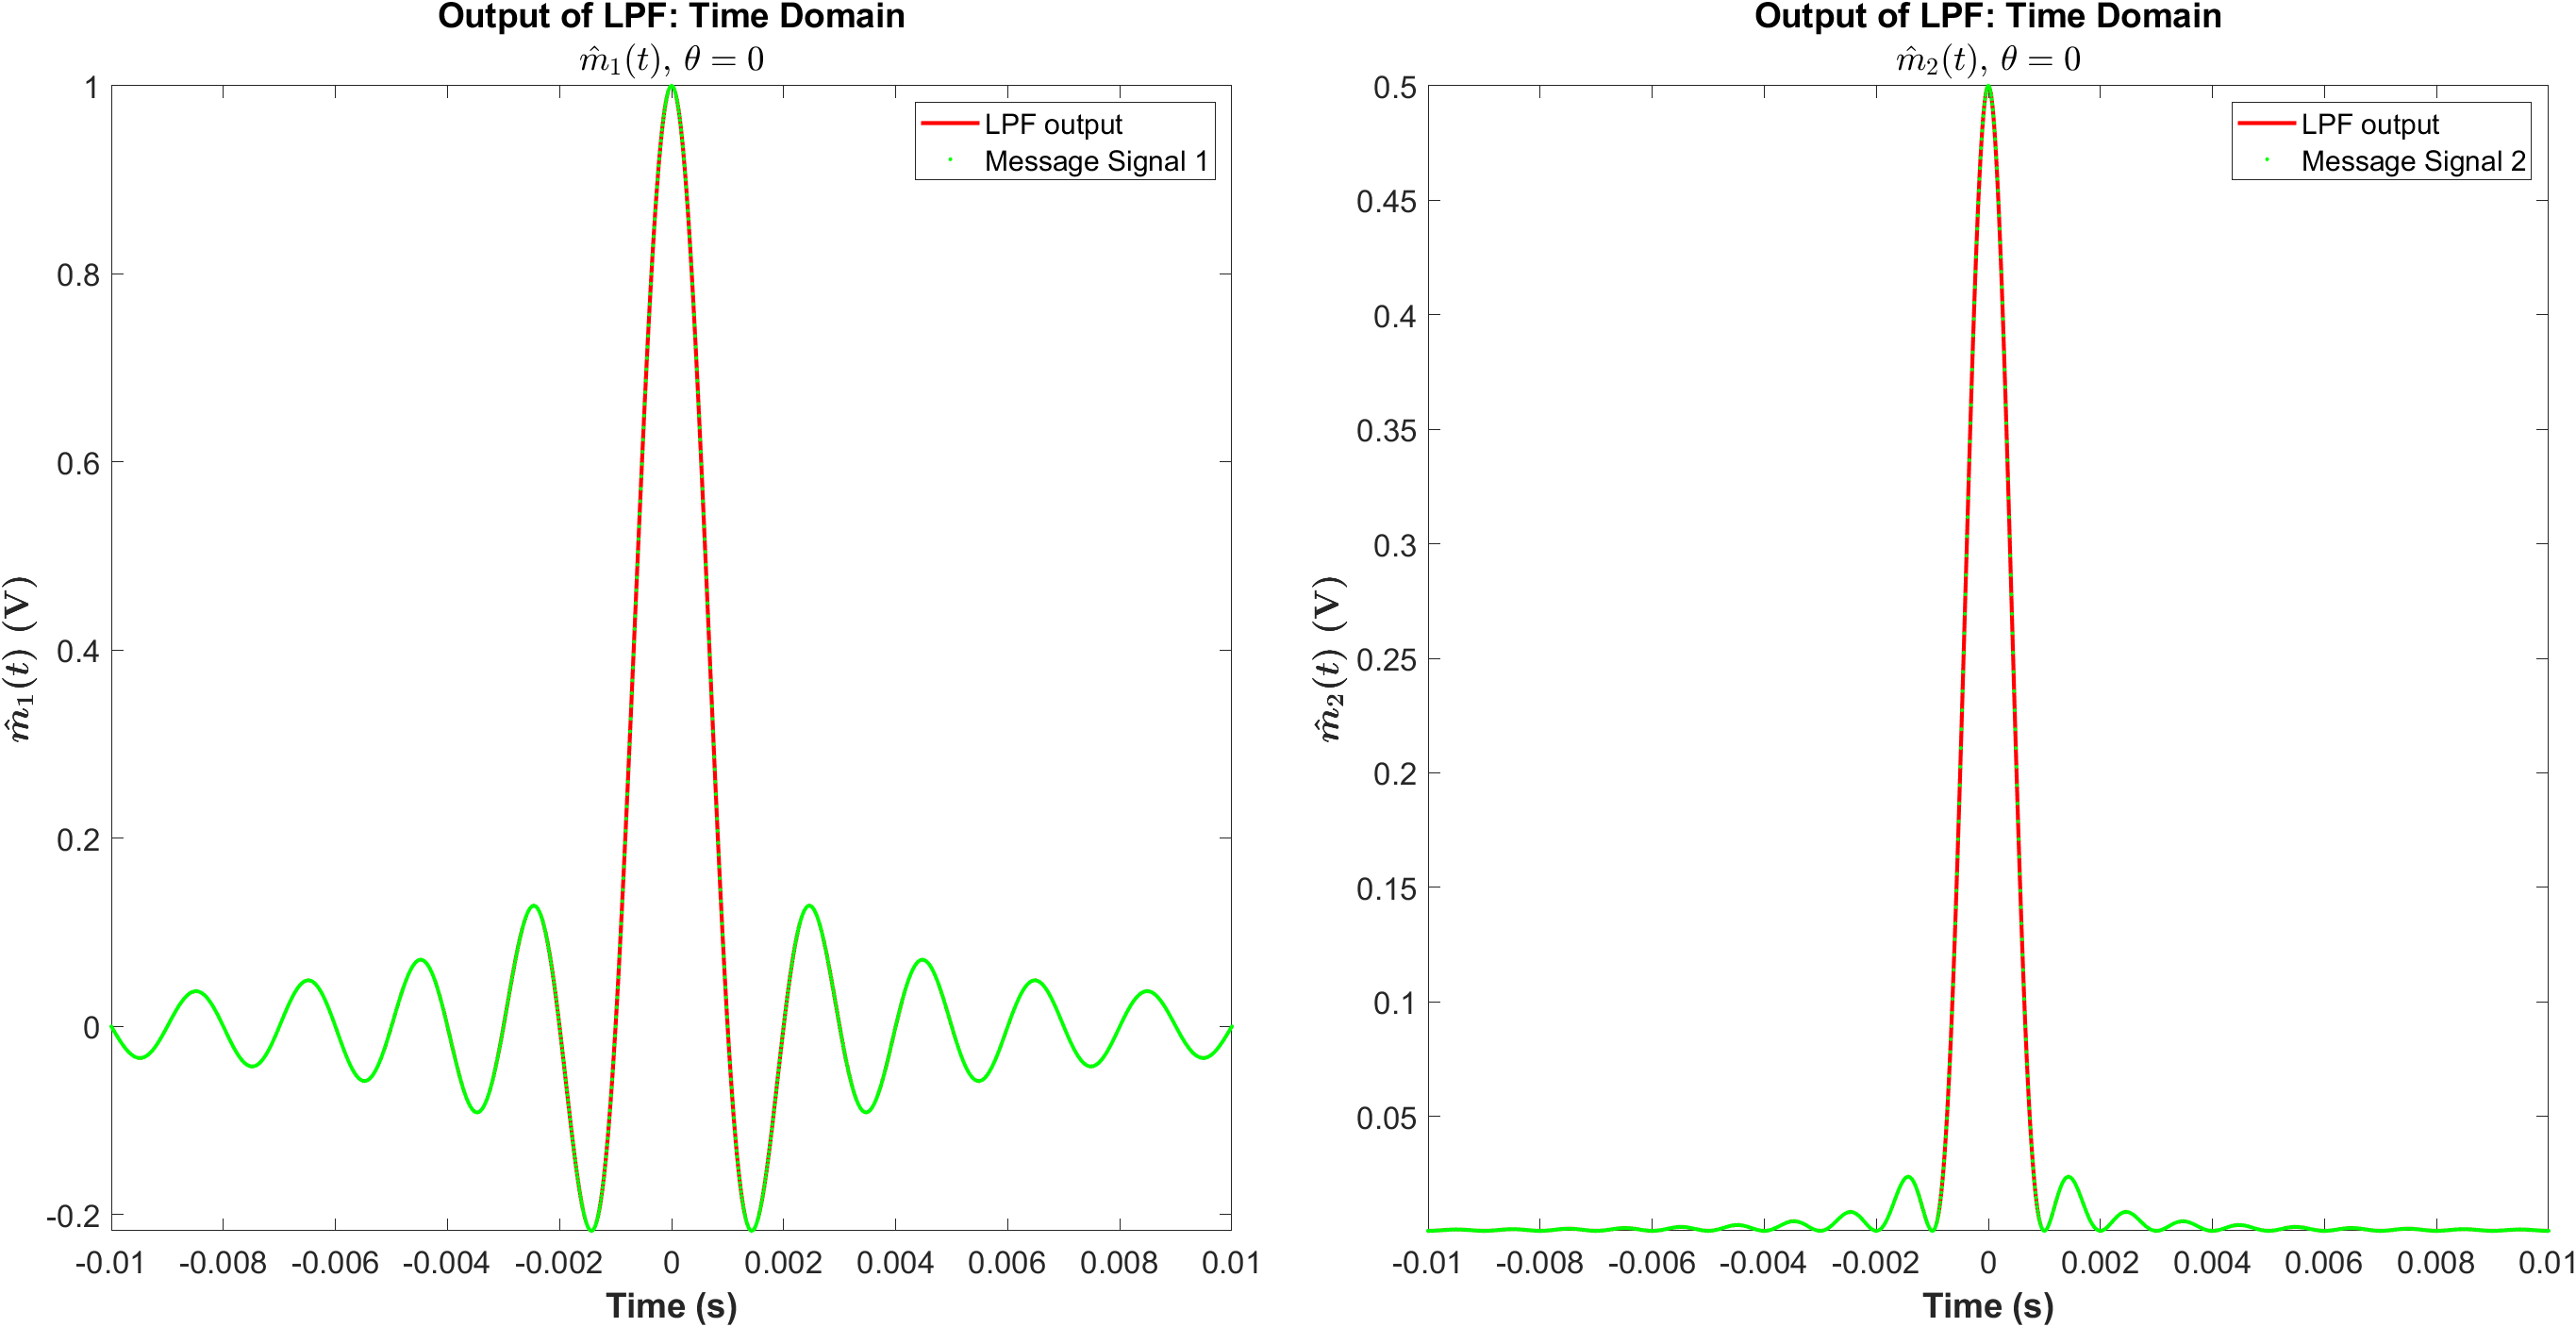
\includegraphics[width=\textwidth]{qam_demod_lpf_theta_0}
    \caption{\label{fig:qam_demod_lpf_0}The QAM Signal in Time Domain}
\end{figure}
\begin{figure}[h]
    \centering
    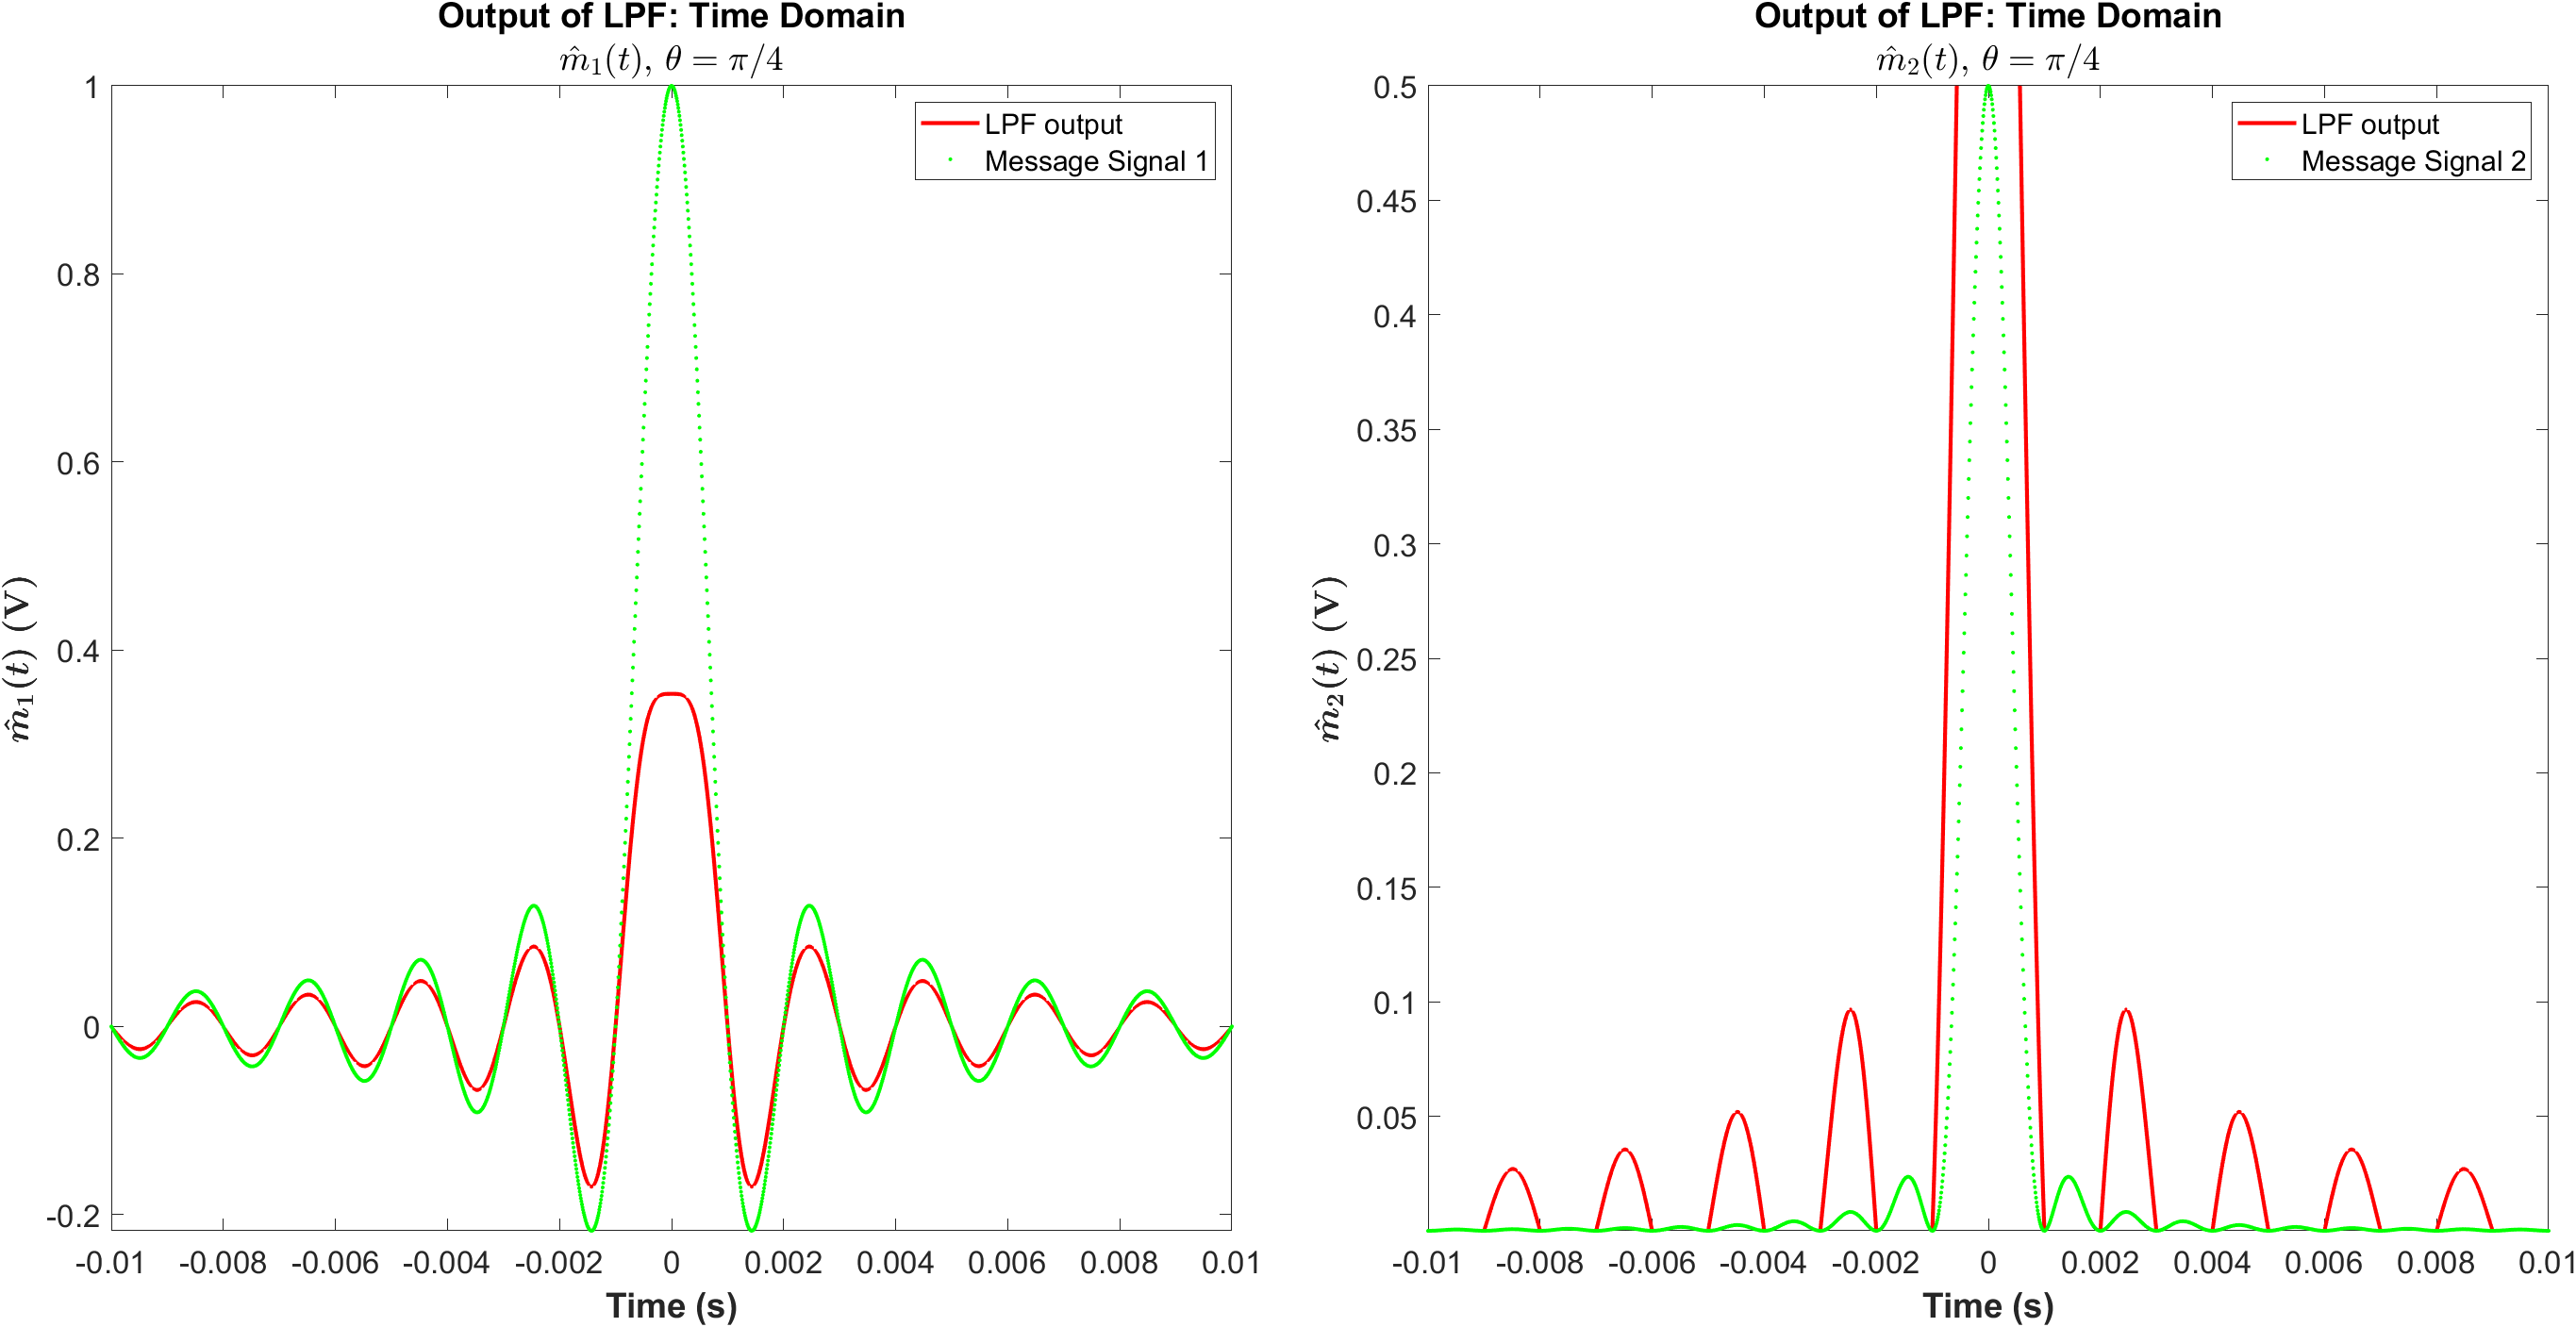
\includegraphics[width=\textwidth]{qam_demod_lpf_theta_0.7854}
    \caption{\label{fig:qam_demod_lpf_p4}The Magnitude Spectrum of the QAM Signal}
\end{figure}

The low-pass filter used for both signals is an ideal low-pass filter with a cut-off frequency of 1.5 kHz. The FFT of the remodulated QAM signal is similar to what occurs with the DSB-SC signal. There are frequency components around the impulses at $\pm f_m$ that we want to filter out, without attenuating the frequency components around $\pm 2f_c \pm f_m$. The possible ranges for the cut-off frequency of the low-pass filter are the same as with the DSB-SC signal, with possible range of cut-off frequencies ranging from slightly above 1 kHz (around 1.3 kHz) to slightly below 19 kHz (around 17.5 kHz). % talk about possible cutoff freq

We can see that when $\theta = 0$, we retrieve the message signal perfectly with no attenuation, while when $\theta = \pi/4$, the message signal is attenuated but can still be retrieved after amplification. This matches our experience with the same $\theta$ values with the DSB-SC signal. 
\end{document}